\chapter{The \texorpdfstring{$\tau_h$}{τh} identification algorithms and their performance}
\label{ch:Tau}
%
The precise and accurate reconstruction of $\tau$ leptons is a crucial part of the $HH\rightarrow bb\tau\tau$ analysis covered in Chapter \ref{ch:bbtt_analysis}. Furthermore, a significant number of physics analyses — such as measurements of Higgs boson production~\cite{CMS-HIG-16-043,CMS-HIG-19-010} and of the \CP structure of its Yukawa coupling to $\tau$ leptons~\cite{CMS-HIG-20-006}, and searches for new physics in final states with $\tau$ leptons~\cite{CMS-HIG-21-001,CMS-PAS-EXO-24-012,CMS-PAS-EXO-24-020} — rely on the adequate identification of $\tau$ decay products and their properties. This broad physics program necessitates continuous development of reconstruction and identification techniques, which in CMS for $\tau$ leptons are coordinated within the Tau Physics Object Group (Tau POG). A central component of the study of $\tau$ leptons, which will be emphasized subsequently, involves validating the applied techniques to ensure their correct behavior in data.

In CMS, the reconstruction and identification of hadronic $\tau$ leptons constitute two complementary steps. The reconstruction stage, performed by the HPS algorithm~\cite{CMS-TAU-14-001} (see Section \ref{subsec:Taus}), assembles the visible decay products into a $\tau_h$ candidate and determines its decay mode and kinematic properties. The identification step then classifies these reconstructed candidates as a genuine $\tau$ lepton or as a misidentified jet, electron or muon.

This chapter provides a detailed examination of the identification of hadronic $\tau$ leptons. Section \ref{sec:Tau_MisID} lays the groundwork and emphasizes the challenges associated with distinguishing genuine $\tau_h$ candidates from background objects, Section \ref{sec:DeepTau2.5} summarizes the identification algorithms and compares their performance, and Section \ref{sec:Tau_validation} presents their validation with the data recorded by CMS from 2022 to 2026. This validation is the contribution of this thesis to the Tau POG, and its results with the 2024 and 2025 data have been published in Ref.~\cite{CMS-DP-2025-074}.


\section{Challenges in \texorpdfstring{$\tau_h$}{τh} identification}
\label{sec:Tau_MisID}
%
As described in Section \ref{subsec:Taus}, the HPS algorithm is configured to prioritize the reconstruction efficiency of genuine $\tau_h$, which exceeds $80\%$ for $p_T > 30$ GeV and approaches $90\%$ above $100$ GeV~\cite{CMS-TAU-20-001}. Therefore, it inevitably suffers from contamination by other processes, meaning that a fraction of reconstructed $\tau_h$ candidates originates from objects that mimic the topology of hadronic $\tau$ decay. The dominant source of misidentification arises from jets, since the HPS algorithm is seeded by PF jets that can reproduce the charged-track multiplicity and electromagnetic signature characteristic of $\tau$ decays, i.e., a highly collimated quark or gluon jet can resemble a $\tau$ decay, as illustrated in Figure \ref{fig:tau_fakes}. Light leptons can also be misidentified as $\tau$ leptons. A muon can mimic a one-prong decay when it deposits a significant fraction of its energy in the calorimeters, while an electron can be taken as the charged hadron of the decay, with the photons it radiates through bremsstrahlung clustered into a strip, which reproduces the signature of a h$^{\pm}\pi^0$ decay. These signatures are also illustrated in Figure \ref{fig:tau_fakes}.
%
% \begin{figure}[h!]
% \centering
% \begin{subfigure}[t]{0.48\linewidth}
%   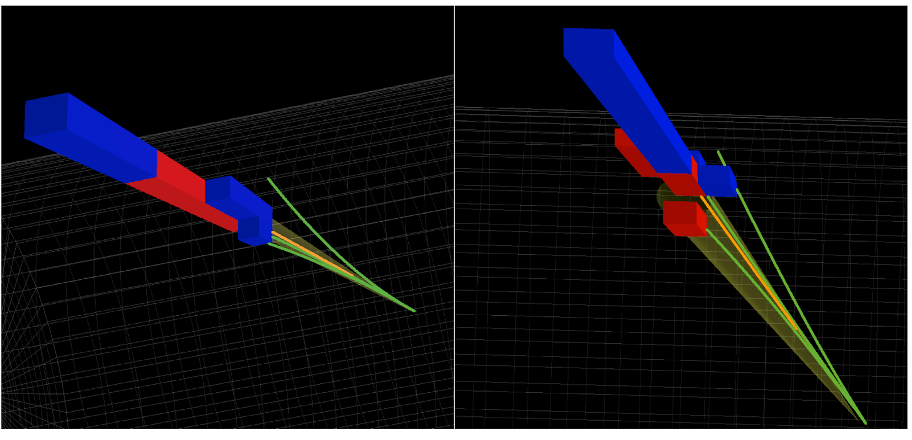
\includegraphics[width=1\linewidth]{figures//chapter_III/tau_jet_sim.png}
%     \caption{Simulation of a $\tau_h$ decay into h$^{\pm}$h$^{\mp}$h$^{\pm}\pi^0$ (left) and of a collimated jet resembling a $\tau_h$ (right) in the CMS detector.}
%     \label{fig:tau_jet_sim}  
% \end{subfigure}
% \hfill
% \begin{subfigure}[t]{0.48\linewidth}
%     \centering
%     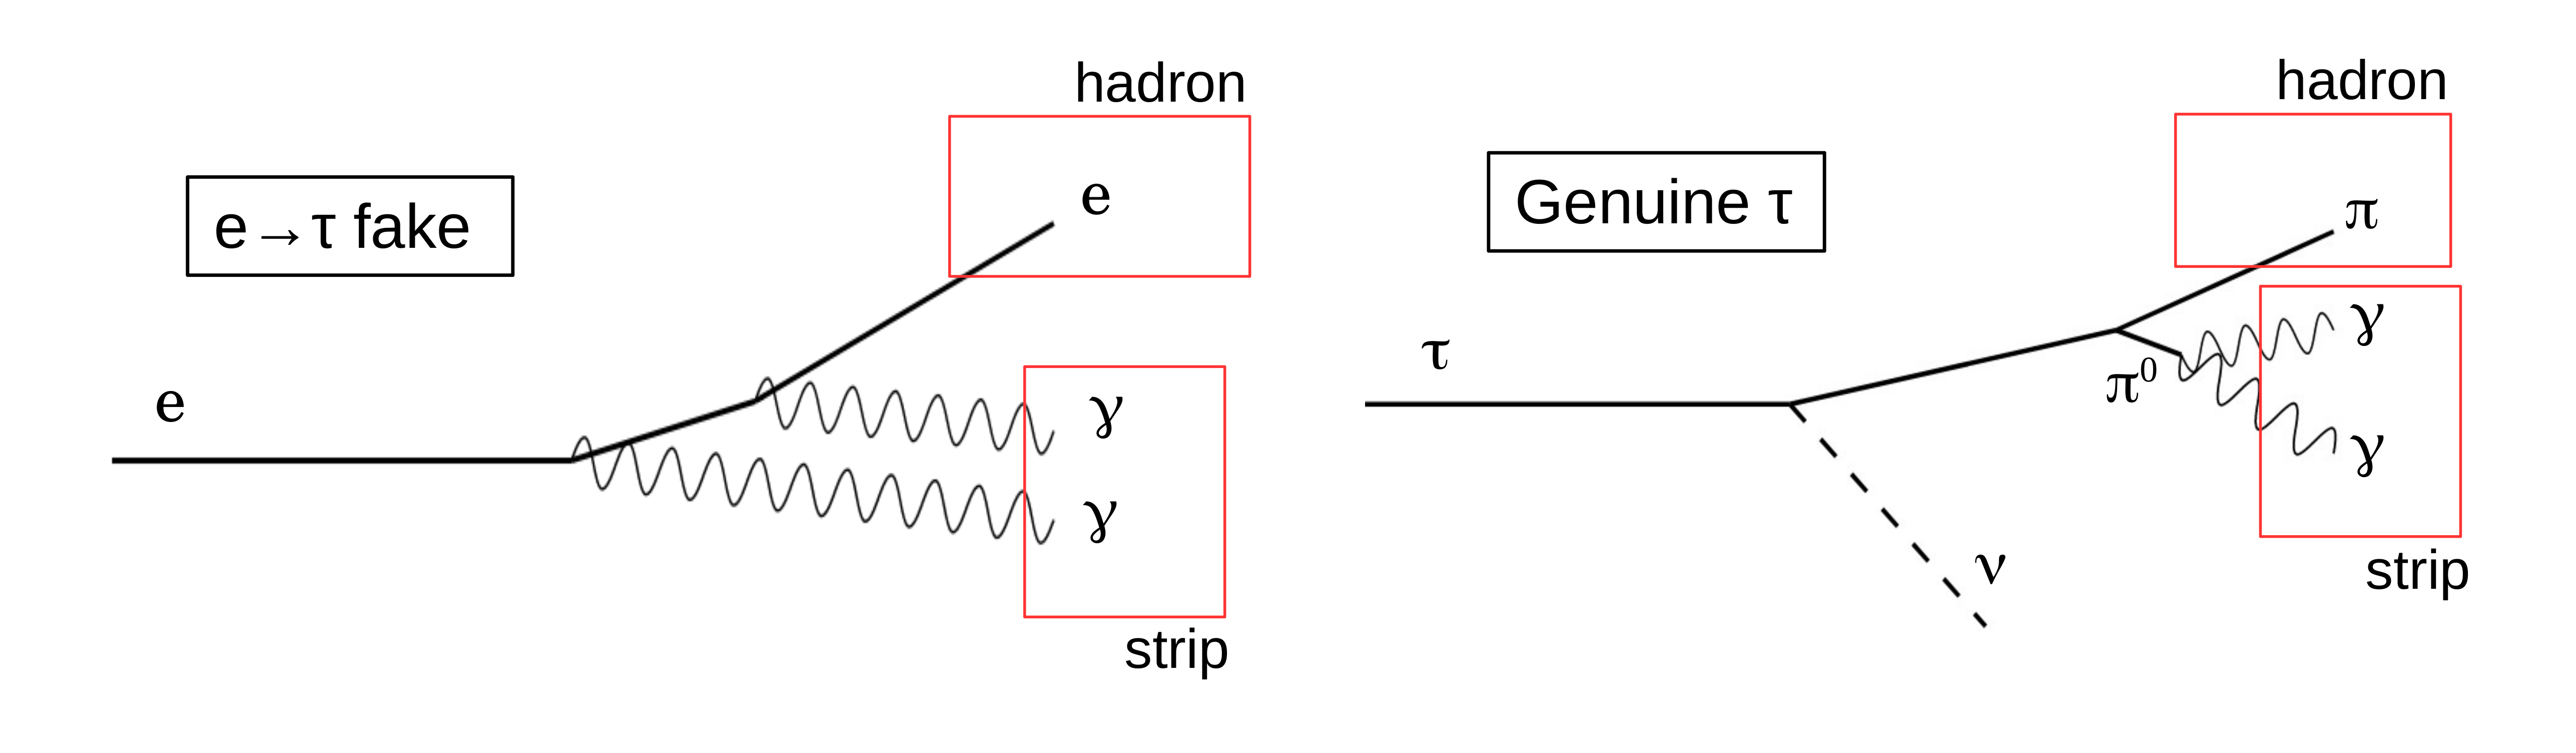
\includegraphics[width=1\linewidth]{figures//chapter_III/electron_faking_tau.png}
%     \caption{Schematic representation of the signatures identified by the HPS algorithm for an electron faking a $\tau_h$ (left) and a genuine $\tau_h$ (right). \textcolor{red}{hacer más grande esta figura}}
%     \label{fig:ele_fake_tau}
% \end{subfigure}
% \caption{Examples of objects misidentified as $\tau_h$ candidates by the HPS algorithm}
% \label{fig:tau_fakes}
% \end{figure}
\begin{figure}[h!]
    \centering
    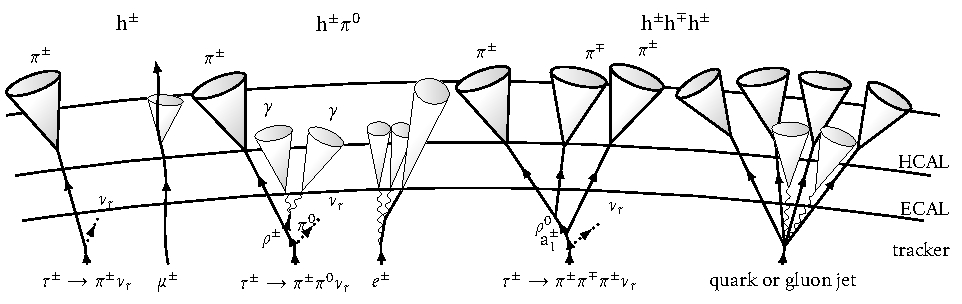
\includegraphics[width=\linewidth]{figures/chapter_III/tau_fakes_tikz.pdf}
    \caption{Signatures of genuine $\tau_h$ decays and of the objects that the HPS algorithm can reconstruct in the same decay mode, indicated above each pair. From left to right, a one-prong decay and a muon that deposits part of its energy in the calorimeters, a one-prong decay with a neutral pion and an electron whose bremsstrahlung photons are clustered into a strip and whose shower reaches the HCAL, and a three-prong decay and a quark or gluon jet, which usually contains more particles spread over a wider angle. Adapted from Ref.~\cite{Neutelings:tau_decay}.}
    \label{fig:tau_fakes}
\end{figure}

The reconstruction of genuine $\tau_h$ has its own limitations. Depending on the decay mode, between $11\%$ (h$^{\pm}$) and $25\%$ (h$^{\pm}\pi^0$) of the generated $\tau_h$ are not reconstructed in any of the HPS decay modes, mainly because the tracks of charged hadrons are reconstructed with an efficiency of about $90\%$~\cite{CMS-TAU-20-001}. Part of the three-prong decays in which one track is lost are recovered as two-prong candidates, but their charge is correctly assigned in only about $70\%$ of the cases, compared with $99\%$ for the other decay modes~\cite{CMS-TAU-20-001}, which is why they are not among the four decay modes used in analyses (Figure \ref{fig:tau_DMs}). These candidates, lost or misreconstructed by HPS, are one of the motivations for the identification algorithms that do not depend on it, presented in Section \ref{subsec:PNet}.

These effects reflect the challenges associated with the complex topology of hadronic $\tau$ decays, and highlight the need for a dedicated identification step to improve the purity of reconstructed $\tau_h$ candidates. To this end, various methods have been implemented in CMS over the years, ranging from cut-based isolation sum discriminators and Boosted Decision Tree discriminator~\cite{CMS-TAU-14-001,CMS-TAU-16-003} to more sophisticated deep learning-based algorithms, described in the following section.


\section{The \texorpdfstring{$\tau_h$}{τh} identification algorithms}
\label{sec:DeepTau2.5}
%
Given the aforementioned reconstruction limitations, a dedicated identification approach is needed. The challenge of discriminating between the reconstructed $\tau_h$ candidates, given the large number of correlated observables involved in this type of task, has led to the adoption of advanced deep learning techniques capable of fully exploiting the available information and ensure robust performance across different data-taking conditions. 

The \textsc{DeepTau} neural network-based algorithm was deployed at the end of Run 2, and has since become the standard $\tau_h$ identification method in CMS. The first version v2.1~\cite{CMS-TAU-20-001} was presented initially, and was then upgraded to v2.5~\cite{CMS-TAU-24-001} during the early Run 3 period, introducing major improvements that will be briefly discussed next. In parallel, alternative identification strategies for genuine $\tau_h$ candidates are being explored, leveraging modern architectures such as graph neural networks (\textsc{PNet}) and transformers (\textsc{UParT}) to treat $\tau_h$ candidates within a broader jet classification framework.



\subsection{The \textsc{DeepTau} algorithm}
\label{subsec:DeepTau}
%
\textsc{DeepTau} is a convolutional neural network that classifies each $\tau_h$ candidate reconstructed by HPS as a genuine $\tau_h$, a quark or gluon jet, an electron or a muon, so that the three discriminations described in Section \ref{sec:Tau_MisID} are performed by a single network~\cite{CMS-TAU-20-001,CMS-TAU-24-001}. To do so, it combines two types of information. The first is a set of high-level variables that describe the candidate as a whole, such as its kinematics, its isolation, or the compatibility of its tracks with the primary vertex. The second is the set of all particles reconstructed around the candidate, whose individual properties are arranged in two grids in the $\eta$-$\phi$ plane centered on the $\tau_h$ axis, an inner grid covering the region of the decay products and a wider outer grid that captures the surrounding activity, which is larger for jets than for genuine $\tau_h$. The input variables of both types are summarized in Table \ref{tab:deeptau_inputs}.
%
\begin{table}[h!]
    \centering
    \begin{tabular}{l l}
        \hline
        \textbf{Input block} & \textbf{Variables} \\
        \hline
        \multicolumn{2}{l}{\textit{High-level features ($43$ variables)}} \\
        $\tau_h$ candidate & $p_T$, $\eta$, energy, charge, number of charged and neutral constituents \\
        Isolation          & energy sums of the different particle types around the candidate \\
        Lifetime           & impact parameters of the leading track, properties of the SV \\
        Strips             & spread in $\eta$ and $\phi$ of the energy in the strips \\
        Electron rejection & calorimeter variables discriminating against electrons \\
        Pileup             & pileup energy density $\rho$ \\
        \hline
        \multicolumn{2}{l}{\textit{Low-level features (inner and outer grids around the $\tau_h$ axis)}} \\
        Particle types     & PF electrons, muons, photons, charged and neutral hadrons, \\
                           & standalone electrons and muons \\
        Kinematics         & $p_T$, $\Delta\eta$ and $\Delta\phi$ with respect to the $\tau_h$ axis, charge \\
        Tracks             & track quality, compatibility with the PV or an SV \\
        Detector deposits  & ECAL and HCAL energy, muon station hits \\
        Pileup             & PUPPI weight \\
        \hline
    \end{tabular}
    \caption{Summary of the input features used by the \textsc{DeepTau} v2.5 algorithm~\cite{CMS-TAU-24-001}.}
    \label{tab:deeptau_inputs}
\end{table}

This set of input information is processed by a combination of dense and convolutional layers, and the final layer of the network acts as a multiclass classifier~\cite{CMS-TAU-20-001}, providing the probabilities that the reconstructed $\tau_h$ candidate corresponds to a genuine $\tau_h$, an electron, a muon, or a quark or gluon jet. From these probabilities, three discriminators are built, one against each type of background (\textsc{VSjet}, \textsc{VSe}, \textsc{VSmu}), by comparing the probability of the genuine $\tau_h$ class with that of the corresponding background. Each discriminator has its own set of working points, defined by the efficiency for genuine $\tau_h$, as described in Section \ref{subsec:Taus}. 

% This set of input information is processed by a combination of dense and convolutional layers, and the final layer of the network acts as a multiclass classifier~\cite{CMS-TAU-20-001}, providing the probabilities that the reconstructed $\tau_h$ candidate corresponds to a genuine $\tau_h$, an electron, a muon, or a quark or gluon jet. From these probabilities, three discriminators are built, one against each type of background (\textsc{VSjet}, \textsc{VSe}, \textsc{VSmu}), defined as
% \begin{equation}
%     D_\alpha = \frac{y_\tau}{y_\tau + y_\alpha}, \qquad \alpha \in \{e,\,\mu,\,\text{jet}\},
%     \label{eq:deeptau_discriminant}
% \end{equation}
% %
% where $y_\tau$ and $y_\alpha$ are the probabilities assigned to the genuine $\tau_h$ class and to the background class $\alpha$, so that $D_\alpha$ approaches unity for genuine $\tau_h$. Each discriminator has its own set of working points, defined by the efficiency for genuine $\tau_h$, as described in Section \ref{subsec:Taus}.
As already mentioned, two versions of \textsc{DeepTau} have been used in CMS. The first, v2.1, was introduced at the end of Run 2 and trained exclusively on simulated events. Its successor, v2.5, used in Run 3 and in the analysis presented in this thesis, keeps essentially the same architecture, but was retrained with a larger and more balanced dataset, optimized hyperparameters and a revised set of inputs. As shown in Figure \ref{fig:DeepTau_versions}, the probability for jets to be misidentified as $\tau_h$ is reduced by $30$–$50\%$ over the whole efficiency range, the rejection of electrons improves mainly for the tightest working points, where the misidentification probability is reduced by almost a factor of two, and the rejection of muons remains unchanged.
%
\begin{figure}[h!]
    \centering
    \begin{subfigure}[t]{0.32\linewidth}
        \centering
        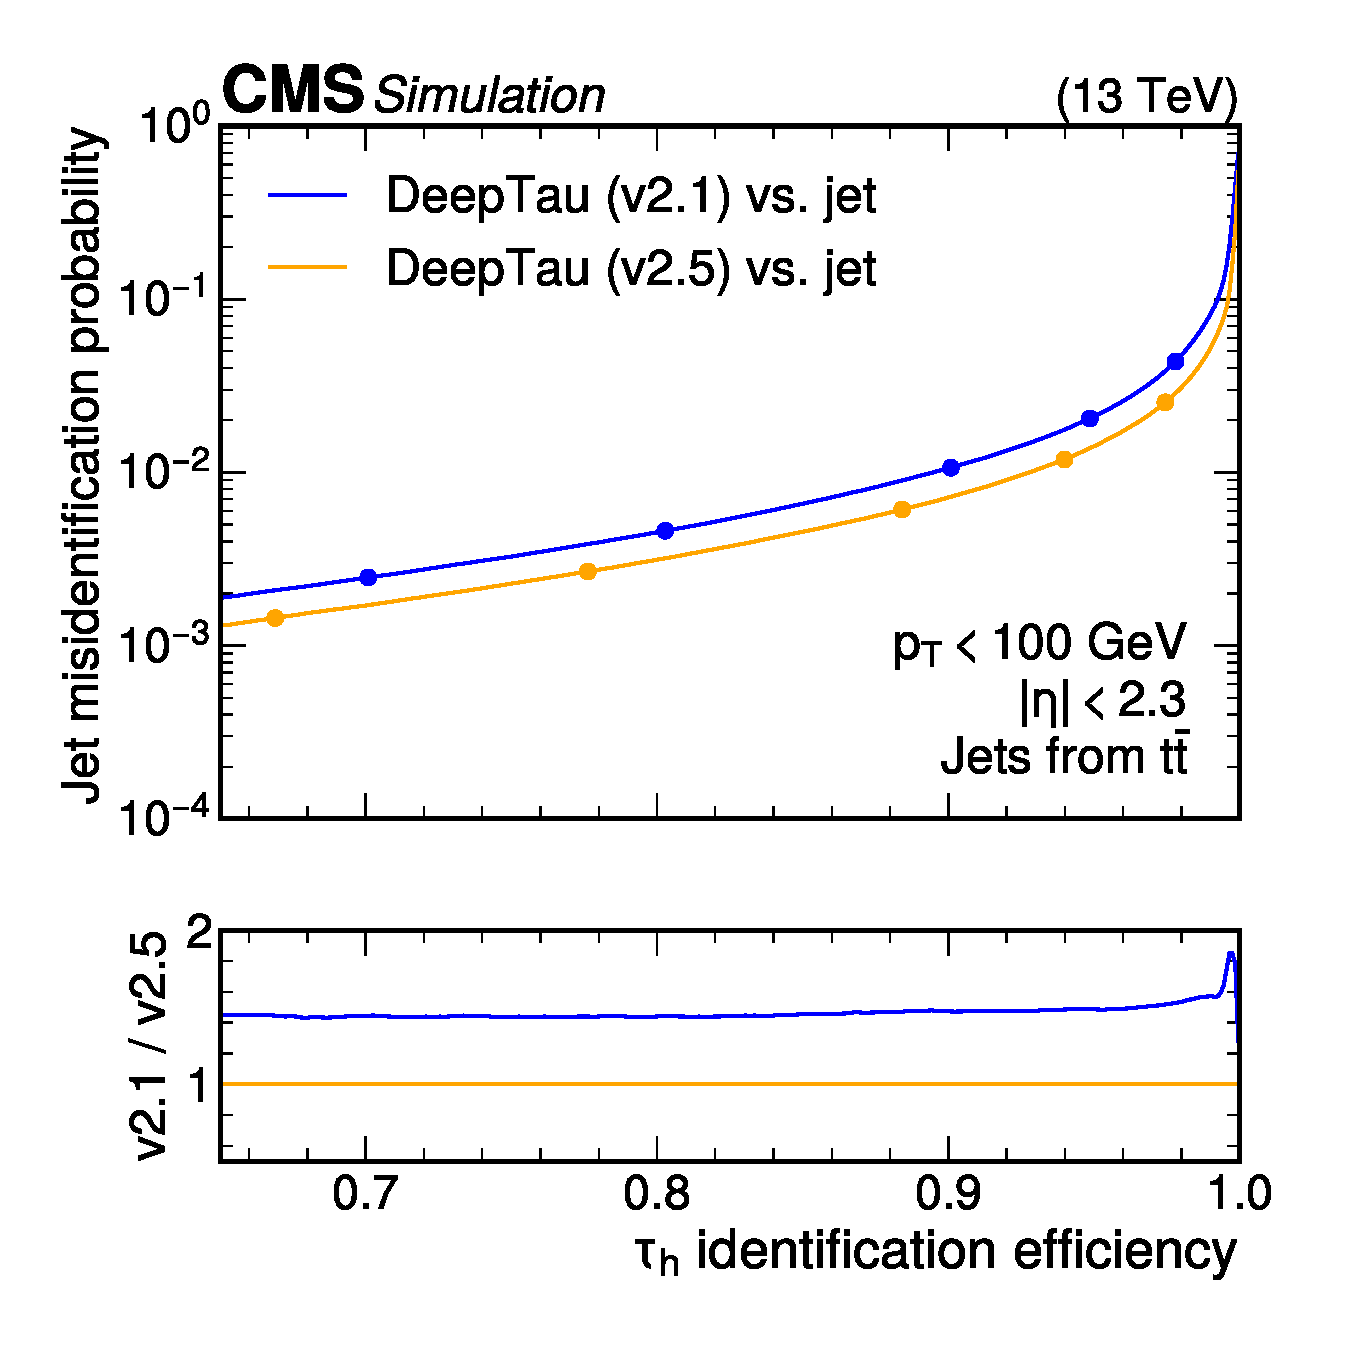
\includegraphics[width=\linewidth]{figures/chapter_III/CMS-TAU-24-001_Figure_006-a.pdf}
        \caption{\textsc{VSjet}}
        \label{fig:DeepTau2p5VSjet}
    \end{subfigure}
    \hfill
    \begin{subfigure}[t]{0.32\linewidth}
        \centering
        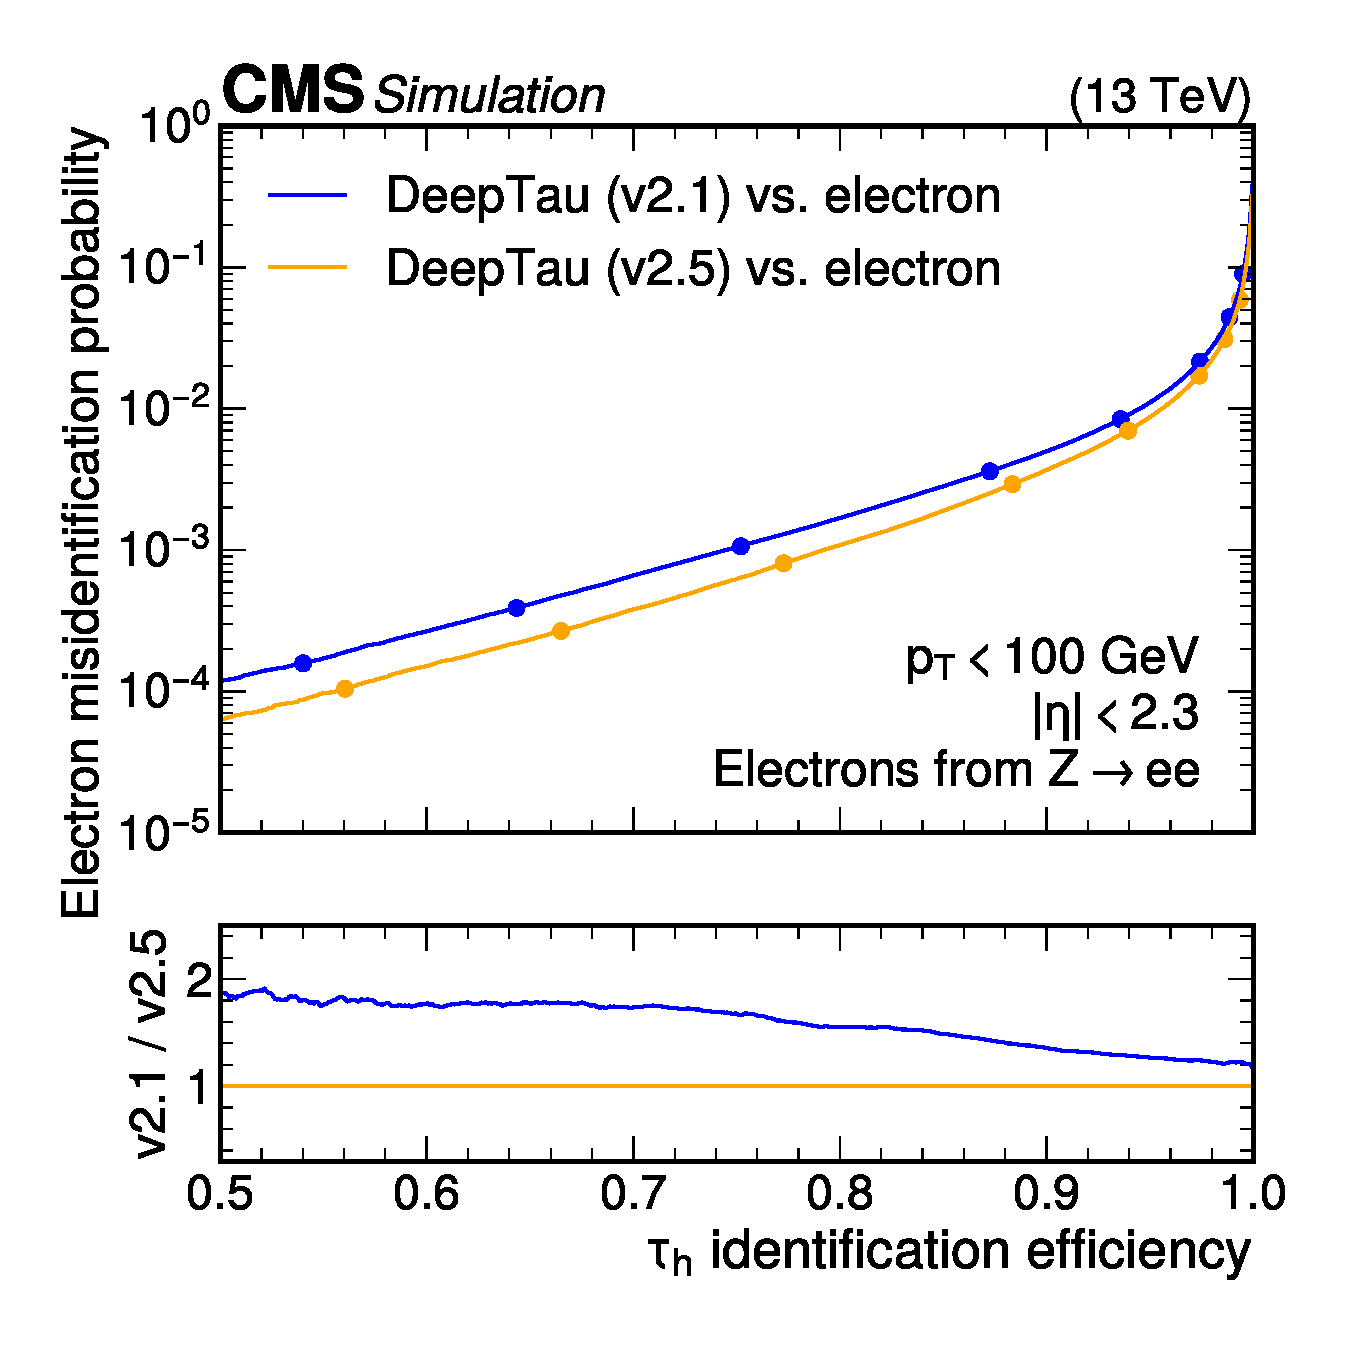
\includegraphics[width=\linewidth]{figures/chapter_III/CMS-TAU-24-001_Figure_007-a.pdf}
        \caption{\textsc{VSe}}
        \label{fig:DeepTau2p5VSe}
    \end{subfigure}
    \hfill
    \begin{subfigure}[t]{0.32\linewidth}
        \centering
        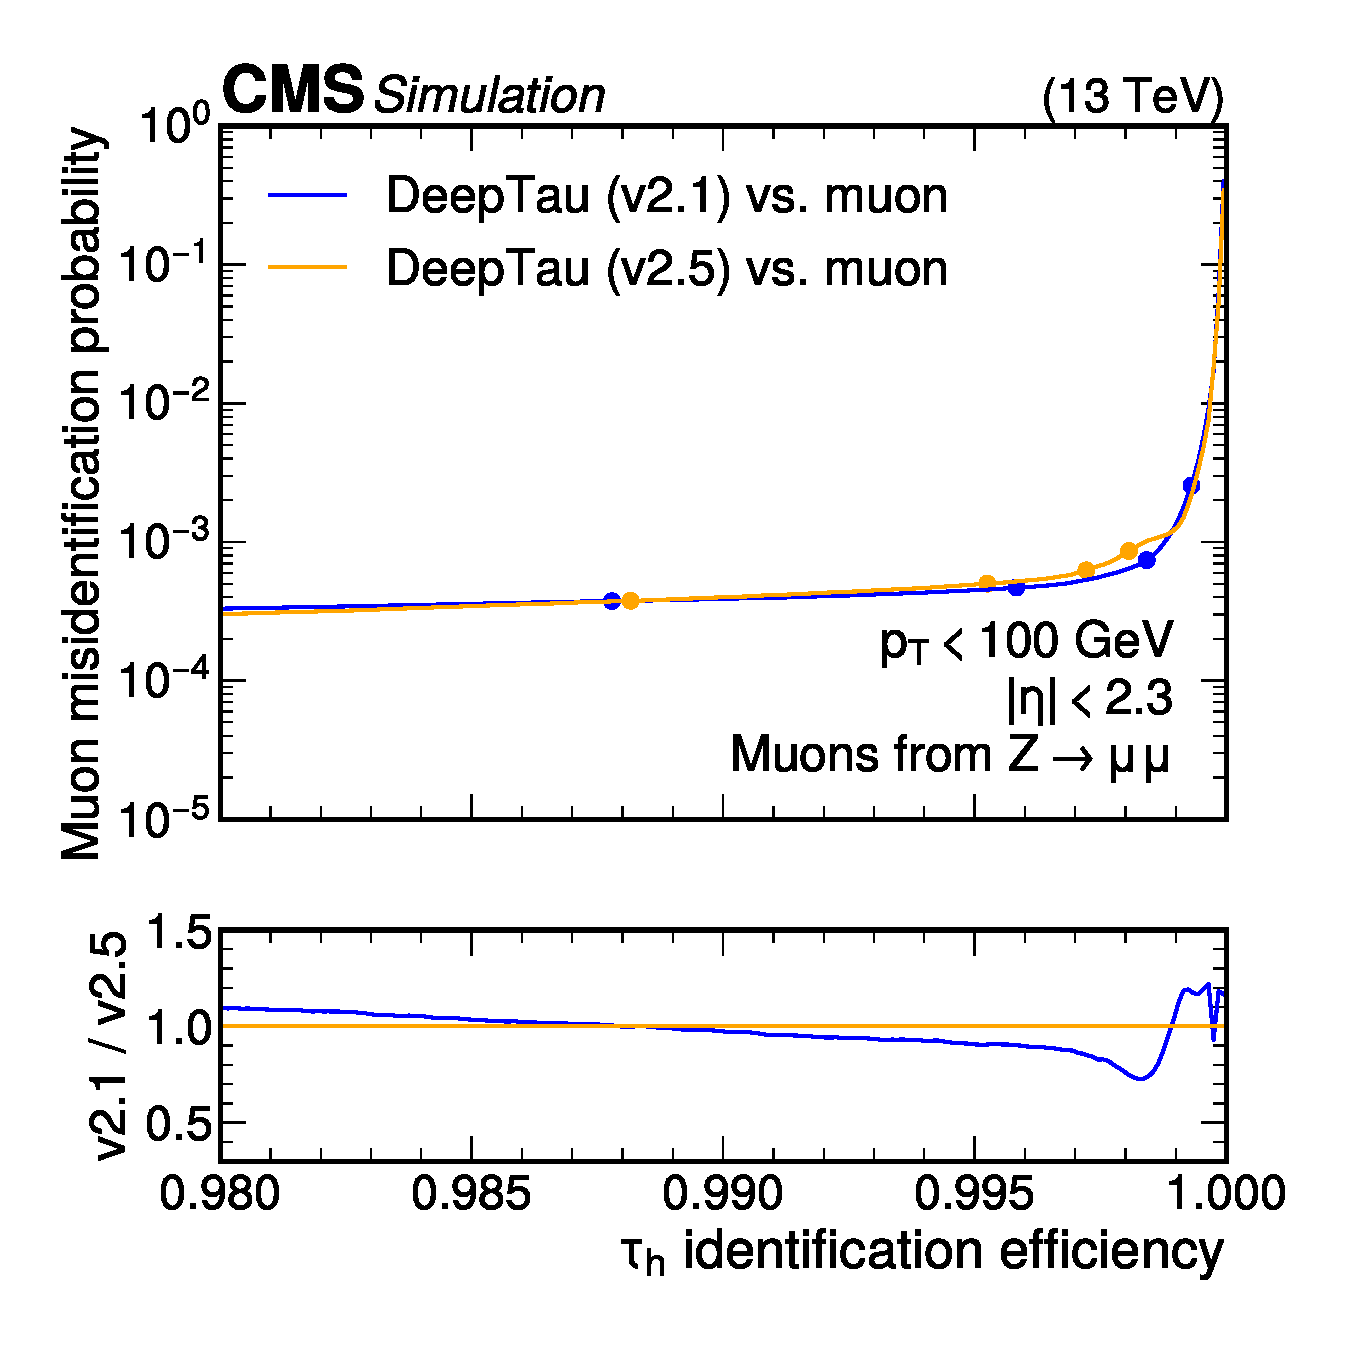
\includegraphics[width=\linewidth]{figures/chapter_III/CMS-TAU-24-001_Figure_008-a.pdf}
        \caption{\textsc{VSmu}}
        \label{fig:DeepTau2p5VSmu}
    \end{subfigure}
    \caption{Misidentification probability of quark and gluon jets (a), electrons (b) and muons (c) as a function of the identification efficiency for genuine $\tau_h$, for the \textsc{DeepTau} v2.1 (blue) and v2.5 (orange) discriminants. The efficiency is evaluated with $H\to\tau\tau$ events and the misidentification probabilities with $t\bar{t}$, $Z\to ee$ and $Z\to\mu\mu$ events, respectively, all simulated with 2018 conditions, for $\tau_h$ candidates with $p_T<100$ GeV and $|\eta|<2.3$. The working points are indicated by filled circles, and the lower panels show the ratio between both versions~\cite{CMS-TAU-24-001}.}
    \label{fig:DeepTau_versions}
\end{figure}

The second novelty of v2.5 is the use of domain adaptation~\cite{CMS-TAU-24-001}. Since v2.1 was trained only on simulation, any mismodeling of its inputs translated into differences between data and simulation in its output. To reduce them, v2.5 is trained on a mixture of simulated events and collision data, so that the network learns to classify $\tau_h$ candidates while avoiding the features that are described differently in data and in simulation. The classification itself is still learned only from simulation, while the collision data come from a sample of $Z\to\tau\tau\to\mu\tau_h$ events rich in genuine $\tau_h$ — the same final state used for the validation in Section \ref{sec:Tau_validation}. As a result, the agreement between data and simulation improves in the highest-score bins, and the corrections that analyses must apply move closer to unity.
%As a result, the agreement between data and simulation improves in the highest-score bins, where the difference in the last bin of the 2018 data used for the training is reduced from $17.4\%$ to $0.9\%$, and also in the 2022 data~\cite{CMS-TAU-24-001}, so that the corrections that analyses must apply move closer to unity.

%


%The corrections are systematically closer to unity for \textsc{v2.5} than for \textsc{v2.1} in both data-taking periods, which confirms the improvement in data-to-simulation agreement brought by the domain adaptation. Their absolute value remains below unity, an effect attributed to the modelling of hadronization and to imperfections in the simulation of the detector alignment and of the track hit reconstruction efficiency~\cite{CMS-TAU-24-001}. The agreement is visibly better for the 2018 dataset, which benefits from an optimized legacy reprocessing and from more mature algorithm calibrations than the early Run-3 data collected in 2022.



%In summary, the use and continuous development of deep-learning algorithms has proven essential for the challenging task of identifying $\tau_h$ leptons. These algorithms effectively complement the HPS reconstruction, yielding highly satisfactory results in background rejection. As a result, these developments significantly reduce the misidentification rate while preserving the efficiency for genuine $\tau_h$ leptons, thereby increasing the overall performance of $\tau$-based analysis.



\subsection{Alternative strategies for \texorpdfstring{$\tau_h$}{τh} identification}
\label{subsec:PNet}
%
In recent years, a different approach to $\tau_h$ identification has emerged in CMS as part of a \textit{unified jet tagging} strategy, in which the $\tau_h$ is treated as one more type of jet, and a single network classifies each jet according to its origin, whether a $b$ quark, a $c$ quark, a light quark, a gluon, an electron, a muon or a hadronically decaying $\tau$ lepton. This approach consistently models the correlations between the identification of the different objects, allows the selection to be optimized against specific sources of contamination, and concentrates computing resources in a single algorithm, used both in the offline reconstruction and in the HLT. Two algorithms follow this strategy, \textsc{ParticleNet} (\textsc{PNet})~\cite{PNet} and the Unified Particle Transformer (\textsc{UParT})~\cite{Qu:2022mxj,CMS-UParT}, both already introduced in Section \ref{subsec:Jets} for the identification of $b$ jets. 


\subsubsection{The Particle Net algorithm}
%
\textsc{PNet} represents the jet as a \textit{particle cloud}, an unordered set of its constituent PF candidates, in contrast with the image in the $\eta$-$\phi$ plane used by \textsc{DeepTau} and with the ordered lists of particles used by \textsc{DeepJet} (Section \ref{subsec:Jets}). This is a natural representation of a jet, whose constituents have no intrinsic order and are distributed irregularly in space. The particle cloud is processed by a graph neural network, a family of architectures suited to sets of elements without a fixed order or geometric structure, in which the features of each particle are updated using those of its nearest neighbors, so that the network learns the relations between the constituents. Unlike \textsc{DeepTau}, whose inputs rely on the intermediate reconstruction performed by HPS, \textsc{PNet} uses only the properties of the individual constituents of the jet, without any previous $\tau_h$-specific reconstruction.

At the time of its introduction, \textsc{PNet} achieved state-of-the-art performance in jet tagging, clearly surpassing the existing methods~\cite{PNet}, and it has since been widely adopted in CMS. Its main application in Run 3, however, has been the identification of $b$ and $c$ jets, for which it was the recommended algorithm in 2022 and 2023 (Section \ref{subsec:Jets}). For $\tau_h$, its use is so far limited to the HLT, where it replaced the online version of \textsc{DeepTau} in 2024 (Section \ref{sec:triggers}), while offline analyses, including the one presented in this thesis, still rely on \textsc{DeepTau}.




\subsubsection{The Unified Particle Transformer algorithm}
%
\textsc{UParT} also represents the jet as a particle cloud, but processes it with a transformer architecture, whose self-attention mechanism weighs the relation between every pair of constituents at once, instead of only between neighbors. Additionally, the \textsc{UParT} algorithm introduces variables that characterize the interaction between jet constituents and secondary vertices, known as pairwise interaction features, enhancing the sensitivity to internal structure of the jet

The first version of \textsc{UParT} was released in 2024~\cite{CMS-UParT}, and an updated version, v2, trained on a dataset twice as large and with a larger network, in 2025~\cite{CMS-DP-2025-081}. As shown in Figure \ref{fig:btag_evolution}, \textsc{UParT} improves on the performance of \textsc{PNet} in the identification of $b$ jets, and it has replaced it as the recommended algorithm for this task since 2024.\medskip



\noindent In both algorithms, the $\tau_h$ is treated as a one more type of jet, and the network returns the probability that the jet belongs to each of the classes considered in the training, which correspond to jets originating from $b$ quarks, $c$ quarks, light quarks and gluons, and to electrons, muons and $\tau_h$ reconstructed as jets, together with a regression of the jet energy~\cite{CMS-UParT}. Therefore, algthough both algorithms were originally designed and customized for AK4 jet classification, they both perform in an inclusive manner heavy flavor and hadronic $\tau$ identification combined with a flavor-aware jet energy and jet resolution regression~\cite{CMS-UParT}. The $\tau_h$ classes are further split according to the charge and the decay mode of the $\tau$ lepton, so that the decay mode of a candidate is not reconstructed from its constituents, as in HPS, but corresponds to the $\tau_h$ class with the highest probability — labeled with the convention of Equation \ref{eq:tau_DM} —, and its charge is obtained in the same way. Since these classes are defined from the generated decay, the networks can separate the h$^{\pm}\pi^0$ and h$^{\pm}\pi^0\pi^0$ modes, which HPS merges into a single decay mode (Section \ref{subsec:Taus}). The class probabilities are then combined into three discriminants against jets, electrons and muons, analogous to those of \textsc{DeepTau} and each with its own set of working points, while the energy regression provides the visible $p_T$ of the $\tau_h$. The whole description of the candidate thus comes from the network itself, without relying on any previous $\tau_h$-specific reconstruction.

Whether these techniques offer a performance competitive with or complementary to that of \textsc{DeepTau} cannot be inferred from their architectures alone, since each algorithm operates on a different reconstructed object, and is assessed in Section \ref{subsec:tau_IDcomparison}. The main features of the three algorithms are summarized in Table \ref{tab:algo_comparison}.
%
\begin{table}[h!]
    \centering\footnotesize
    \begin{tabular}{l l l l}
        \hline
         & \textbf{HPS+\textsc{DeepTau}} & \textbf{CHS+\textsc{PNet}} & \textbf{PUPPI+\textsc{UParT}} \\
        \hline
        Input object      & HPS $\tau_h$ candidate & AK4 jet & AK4 jet \\
        Inputs            & high- and low-level & low-level & low-level \\
        Representation    & $\eta$-$\phi$ grids & particle cloud & particle cloud \\
        Architecture      & CNN & graph NN & transformer \\
        Relations between & neighboring cells & nearest neighbors & all pairs, with \\
        constituents      &                   &                   & pairwise features \\
        Decay mode        & HPS (DMs $0$, $1$, $10$, $11$) & network (DMs $0$, $1$, $2$, $10$, $11$) & network (DMs $0$, $1$, $2$, $10$, $11$) \\
        Charge            & HPS & network & network \\
        Outputs           & \textsc{VSjet}, \textsc{VSe}, \textsc{VSmu} & jet flavor and $\tau_h$ classes, & jet flavor and $\tau_h$ classes, \\
                          &                                             & $p_T$ regression & $p_T$ regression \\
        \hline
    \end{tabular}
    \caption{Summary of the main features of the three $\tau_h$ identification algorithms compared in this chapter.}
    \label{tab:algo_comparison}
\end{table}




%Thus, as a particle-cloud tagger, the algorithm uses information directly from the PF candidates — which constitute the elements of the cloud — and is trained using low-level inputs and their correlations. Additionally, the \textsc{UParT} algorithm introduces variables that characterize the interaction between jet constituents and secondary vertices, known as pairwise interaction features, enhancing the sensitivity to internal jet structure. The transformer architecture provides greater flexibility for capturing global patterns, thereby complementing the description based on particle interactions characteristic of graph-based approaches such as~\textsc{PNet}.






\subsection{Comparison between \texorpdfstring{$\tau_h$}{τh} identification algorithms}
\label{subsec:tau_IDcomparison}
%DP2025-073 
To understand the complementarity of the described algorithms for identifying hadronic $\tau$ leptons based on advanced ML techniques, the subsequent section presents a comparison of the performance of each of them: \textsc{DeepTau v2.5}, \textsc{PNet} and \textsc{UParT v2}. The comparison will be made in terms of efficiency in the reconstruction and identification of genuine $\tau_h$ versus the ability to reject misidentified objects, as well as the accuracy in classifying $\tau$ decay modes, with the aim of discerning the strenghts of each algorithm and understanding how they complement one another. 

As previously discussed, a key distinction between the algorithms lies in the neural network architectures they exploit to perform the identification. However, this task requires the use of different reconstructed objects as input for each respective algorithm. To ensure a valid comparison, it is essential to consider the distinct reconstructed objects on which each algorithm operates. As indicated previously, \textsc{DeepTau} operates directly on HPS $\tau_h$ candidates; \textsc{PNet} and \textsc{UParT}, on the other hand, are fed AK4 jets that have been reconstructed by CMS taking into account the subtraction of pileup particles using dedicated algorithms, described in Section \ref{subsec:Jets}: charged-hadron substraction (CHS) and pileup-per-particle identification (PUPPI). Therefore, given the varying reconstruction efficiencies of these objects, a unified collection of $\tau$ candidates is defined, obtained as the union of HPS $\tau$ candidates, CHS jets, and PUPPI jets, to which a very loose selection is applied.

Accordingly, the performance of the classifiers is evaluated by taking into account the reconstruction efficiency of their associated reconstruction algorithm. This evaluation is based on ROC curves that show the fraction of no-$\tau_h$ objects that pass the discriminant (misidentification probability) compared to the fraction of genuine $\tau_h$ from the unified collection that pass the discriminant (efficiency) for each individual discriminant: \textsc{VSjet}, \textsc{VSe} and \textsc{VSmu}. This is depicted in Figure \ref{fig:ROC_tauID}, which demonstrates the performance of each discriminant for quark and gluon jets, electrons, and muons misidentified as $\tau_h$ using HPS+\textsc{DeepTau} (blue in the figure), CHS+\textsc{PNet} (yellow), PUPPI+\textsc{PNet} (red), and PUPPI+\textsc{UParT} (purple), where the solid markers indicate the respective working points. As illustrated in Figure \ref{fig:ROC_tauID}, the intrinsic efficiency of the HPS reconstruction is approximately \textcolor{red}{70\%}, and it can be easily recovered using \textsc{PNet}/\textsc{UParT}. The ROC curves also yield different conclusions depending on the discriminant evaluated. Thus, for discrimination agains quark and gluon jets, CHS+\textsc{PNet} demonstrates the most optimal global performance, with HPS+\textsc{DeepTau} offering a close second in the high-purity regime, configuration frequently employed in analyses; whereas in discrimination against electrons and muons, \textsc{UParT} emerges as the leader in performance, with HPS+\textsc{DeepTau} ranking second in the high-purity regime.

UParT achieves the best performance, followed by HPS+DeepTau in high-rejection mode, where its efficiency is not limited by the inefficiency of the HPS reconstruction.

The comparison must be read along two different axes. At a fixed efficiency within the
range accessible to all algorithms, the performances are comparable: CHS+\textsc{PNet}
provides the lowest jet misidentification rate, reducing it by 15--25\% with respect to
HPS+\textsc{DeepTau}, whereas PUPPI+\textsc{UParT} performs worse than
HPS+\textsc{DeepTau} against jets and clearly better against electrons and muons. The
qualitative difference appears instead in the accessible range: HPS+\textsc{DeepTau}
saturates at a $\tau_h$ efficiency of about 70\%, set by the HPS reconstruction itself,
while the jet-based taggers extend up to approximately 90\%, recovering candidates that HPS
does not reconstruct at all.


\begin{figure}[htbp]
    \centering
    
    \begin{subfigure}{0.32\textwidth}
        \centering
        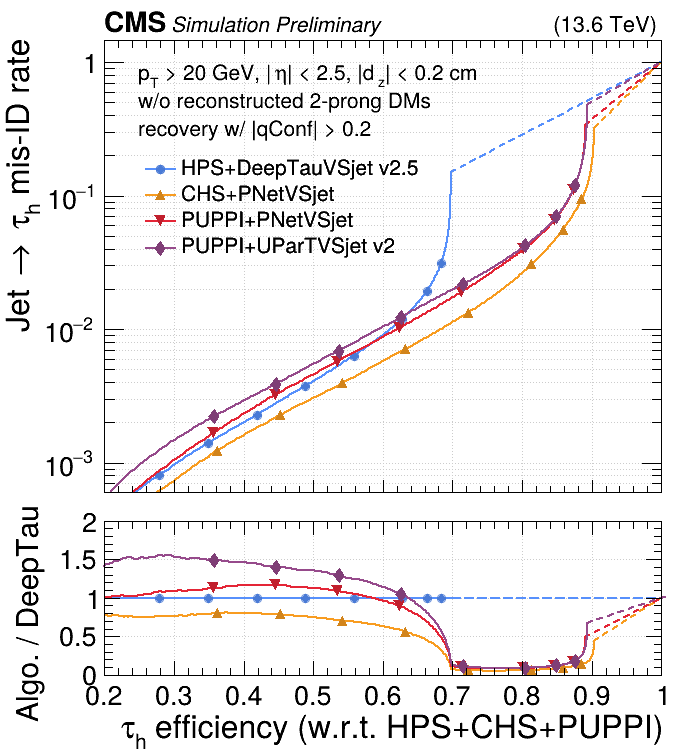
\includegraphics[width=\linewidth]{figures/chapter_III/ROC_IDvsJET.png}
        \caption{\textsc{VSjet}}
    \end{subfigure}
    \hfill
    \begin{subfigure}{0.32\textwidth}
        \centering
        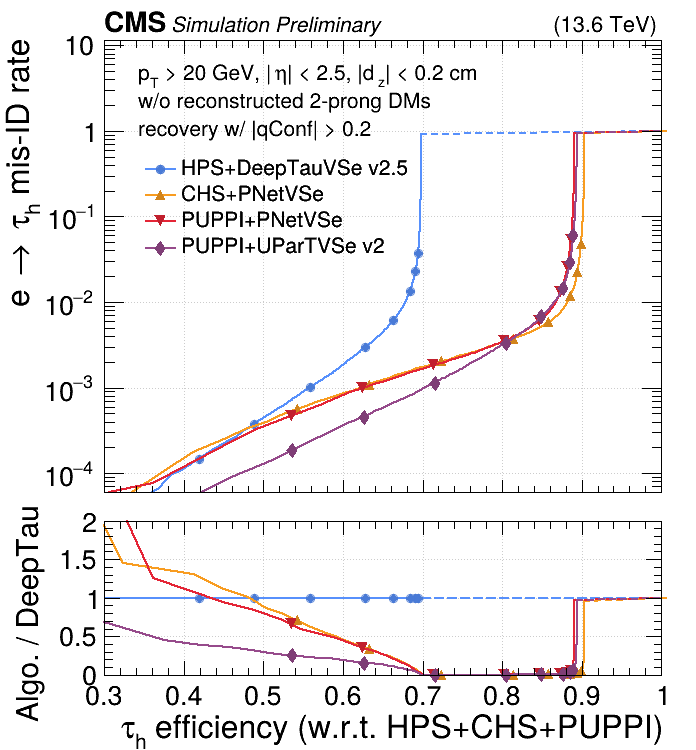
\includegraphics[width=\linewidth]{figures/chapter_III/ROC_IDvsE.png}
        \caption{\textsc{VSe}}
    \end{subfigure}
    \hfill
    \begin{subfigure}{0.32\textwidth}
        \centering
        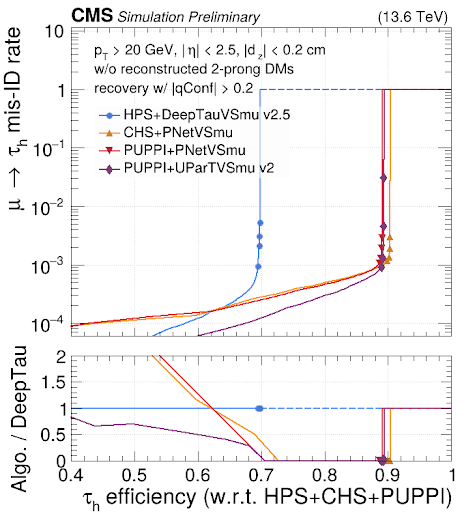
\includegraphics[width=\linewidth]{figures/chapter_III/ROC_IDvsMU.png}
        \caption{\textsc{VSmu}\textcolor{red}{ calidad de imagen}}
    \end{subfigure}
    
    \caption{ROC curves illustrating the performance of the \textsc{DeepTau}, \textsc{PNet}, and \textsc{UParT} algorithms to discriminate quark and gluon jets (a), electrons (b) and muons (c) misidentified as $\tau_h$ candidates. The efficiencies are evaluated taking into account the preceding reconstruction and pileup mitigation algorithms used, labeled HPS, CHS, and PUPPI. Extracted from \textcolor{red}{ref}}
    
    \label{fig:ROC_tauID}
\end{figure}

The key finding from this comparison is the competitive performance of these algorithms across various scenarios. Therefore, the subsequent concern to be adressed is the overlap between the $\tau_h$ candidates identified by each algorithm.

This is illustrated in Figure \ref{fig:venn_combined}, which displays the overlap and complement between $\tau_h$ candidates from the various reconstruction and identification combinations for the described algorithms. This behavior is represented graphically via Venn diagrams, which present the proportion
of candidates identified exclusively by each algorithm or concurrently by multiple algorithms following the application of the Medium WP of the discriminant \textsc{VSjet}. It has been determined that CHS+\textsc{PNet} and PUPPI+\textsc{UParT} can successfully recover between 24-32\% of genuine $\tau_h$ candidates that have not been reconstructed by the HPS algorithm or identified by \textsc{DeepTau}. However, it should be noted that these recovered candidates are more likely to be misidentified jets. This illustrates the complementary nature of the algorithms: while \textsc{DeepTau} maintains high purity, \textsc{PNet} and \textsc{UParT} demonstrate highly efficient performance capable of recovering lost candidates.


\begin{figure}[h!]
    \centering

    \begin{subfigure}[t]{0.48\linewidth}
        \centering
        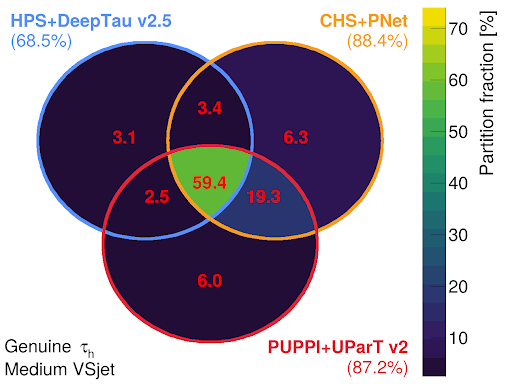
\includegraphics[width=\linewidth]{figures/chapter_III/Venn_1.png}
        \caption{Genuine $\tau_h$ candidates}
        \label{fig:venn1}
    \end{subfigure}
    \hfill
    \begin{subfigure}[t]{0.48\linewidth}
        \centering
        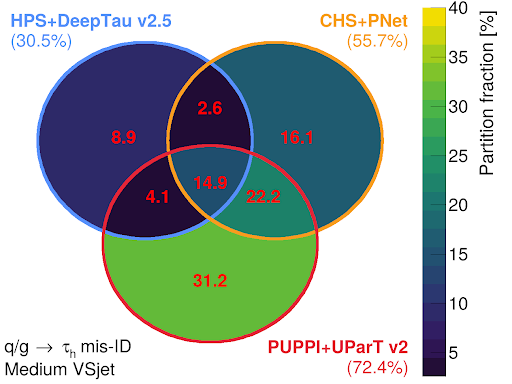
\includegraphics[width=\linewidth]{figures/chapter_III/Venn_2.png}
        \caption{Quark and gluon jets misidentified as $\tau_h$}
        \label{fig:venn2}
    \end{subfigure}

    \caption{Venn diagrams illustrating the overlap and complement between $\tau_h$ candidates from the HPS+\textsc{DeepTau} (blue circle), CHS+\textsc{PNet} (orange circle) and PUPPI+\textsc{UParT} (red circle) algorithms for genuine $\tau_h$ candidates (a) and jets misidentified (b). The red number and fill color of each partition indicate the fraction of candidates it contains relative to the union of all partitions in the diagram. Extracted from \textcolor{red}{ref}}
    \label{fig:venn_combined}
\end{figure}

\textsc{PNet} and \textsc{UParT} have been shown to outperform in terms of $\tau_h$ recovery. Additionally, in terms of decay mode assignment, they both exhibit superior capability compared to the HPS algorithm, as they provide finer resolution in the separation of decay modes and distinguish between the $h^{\pm}\pi^0$ and $h^{\pm}\pi^0\pi^0$ DMs, which were merged by HPS.\medskip


Overall, the revised comparison indicates that the performance of the algorithms varies across misidentified objects and in their description of the internal structure of the $\tau_h$ candidate. Each of the classifiers has been found to have different strengths. \textsc{PNet} provides the best rejection of misidentified quark and gluon jets, while \textsc{DeepTau v2.5} and \textsc{UParT v2} provide the best rejection of misidentified electrons and muons. When it comes to assign the DM, \textsc{PNet} and \textsc{UParT v2} show overall superiority. This underscores the potential value of exploring diverse machine learning architectures in enhancing $\tau_h$ candidate identification, and the efficacy of combining these architectures to achieve the most advanced $\tau_h$ identification to date.

% Finally, it should be noted that while this text has focused on standard CMS strategies, additional algorithms have been developed to target topologies not adequately covered by standard reconstruction and identification techniques. These additional algorithms are briefly mentioned below: \textsc{DisTau} \textcolor{red}{ref}, used to identify $\tau_h$ candidates that have been produced displaced from the primary interaction vertex; \textsc{Boosted DeepTau} \textcolor{red}{ref}, specially designed for $\tau_h$ candidates that have been produced as part of a boosted $\tau\tau$ system; and a modified version of HPS algorithm tailored to low-$p_T$ $\tau_h$ candidates \textcolor{red}{ref}, accompanied by a dedicated energy flow neural network called \textsc{TauNet} \textcolor{red}{ref}. \cite{CMS-DP-2025-047}

\section{Performance with \texorpdfstring{$\sqrt{13.6}$}{√13.6} TeV data}
\label{sec:Tau_validation}

Validating the performance of the algorithms presented for reconstructing and identifying $\tau_h$ in real data is an essential step in ensuring the reliability of any physics analysis using hadronic $\tau$ particles. Therefore, although the algorithms detailed in the previous section have been extensively optimized and evaluated in simulations, it is imperative to verify their performance in each data run conducted by CMS, and, by doing so, monitor the behavior of the techniques developed and actually used in analyses under real experimental conditions.

As part of this thesis work, the $\tau_h$ reconstruction and identification performance of these algorithms has been systematically validated within the Tau POG by evaluating data from all years of Run-3, covering the data-taking periods from 2022 through early 2026. The following sections present two fundamental aspects of this validation. First, Section \ref{subsec:Data-MC-agreement} presents the results in terms of Data to MC comparison for all the aforementioned data-taking periods, which resulted in an internal CMS Detector Performance note \textcolor{red}{DP-2025-074}. Second, Section \ref{subsec:TES_checks} addresses the stability and consistency of performance across the different years of data collection and, consequently, across the changing conditions of the detector. \textcolor{red}{invertir el orden? hablar primero de stability de los datos y luego data-to-MC?}


\subsection{Data-to-MC comparison in Run-3}
\label{subsec:Data-MC-agreement}

To evaluate the performance of the $\tau_h$ modeling in CMS, the simulation is compared with data collected during different data-taking periods for various distributions of relevant variables. The simulation utilized for the comparison is based on the Summer24 NanoAODv15 campaign, which serves as the most up-to-date reference, incorporating the variables required for the recent \textsc{PNet} and \textsc{UParT v2} models. The Monte Carlo (MC) simulation is validated using data from all years of Run-3 processed (or reprocessed in the case of data collected during 2022 and 2023) within the same NanoAODv15 campaign, ensuring consistency between the comparison. 

The simulated samples include the main processes contributing to the selected final state: Drell-Yan, top quark pair production, W+jets, and di-Boson processes. The simulation is partially calibrated to describe the data, including corrections unrelated to the $\tau$ particles, such as calibration of the number of pileup interactions, corrections to the $t\bar{t}$ system momentum and $Z$ boson transverse momentum spectra, and correction factors for muon identification and isolation efficiency. Multijet QCD contribution, which is challenging to model in simulation, is estimated directly from the data in a sideband region adjacent to that used in the validation, and is extrapolated to the signal region.

%\textcolor{red}{No dar tanto detalle?}
%To ensure the accuracy of the validation, events in both data and MC simulations are selected within a well-controlled region enriched in $Z\rightarrow \tau\tau \rightarrow \mu \tau_h$ events using a combination of triggers to select muons with $p_T>24$ GeV. A series of selection criteria is the applied to the $\mu$ and $\tau$ candidates, as briefly described in the following. First, both candidates must have opposite electric charges to ensure that the selected topology is compatible with the $Z\rightarrow \tau\tau$ decay and to suppress other background contributions. The $\mu$ is selected using standard CMS cuts: $p_T>26$ GeV, $|\eta|<2.4$, isolation $<0.15$, and the Medium Working Point for the Muon ID in CMS \textcolor{red}{ref}. The $\tau$ is selected with $p_T > 20$ GeV and $|\eta|<2.5$, and it satisfies the following Working Points corresponding to \textsc{DeepTau v2.5}: VVLoose \textsc{VSe}, Tight \textsc{VSmu}, and Medium \textsc{VSjet}, corresponding to reconstruction efficiencies of 99\%, 99.5\% y 70\% respectively. This selection is replaced by an analogous one for the \textsc{PNet} and \textsc{UParT v2} algorithms. Finally, to define the enriched region in $Z\rightarrow \tau\tau \rightarrow \mu \tau_h$, a cut is made on the transverse mass in the muon - Missing Transverse Energy (MET) system, $m_T(\mu,MET)$, requiring $m_T(\mu,MET)<65$ GeV, as illustrated in Figure \ref{fig:mT_cut_baseline}. This is motivated to exclude

To guarantee the precision of the validation, events in both data and MC simulations are selected within a well-controlled region enriched in $Z\rightarrow \tau\tau \rightarrow \mu \tau_h$ events using data collected with muon triggers. A series of standard selection criteria is applied to the $\mu$ and $\tau$ candidates, which will not be detailed, to ensure a well-reconstructed set of objects. To facilitate reliable identification performance, the $\tau_h$ must satisfy the following Working Points (WPs) in accordance with \textsc{DeepTau v2.5}: VVLoose \textsc{VSe}, Tight \textsc{VSmu}, and Medium \textsc{VSjet}, corresponding to reconstruction efficiencies of 99\%, 99.5\% y 70\% respectively. This selection is replaced by an analogous one for the \textsc{PNet} and \textsc{UParT v2} algorithms, aiming at keeping the same yield for the $Z\rightarrow \tau\tau \rightarrow \mu \tau_h$ process. To define the region enriched in $Z\rightarrow \tau\tau \rightarrow \mu \tau_h$, a requirement is imposed on the transverse mass in the muon - $p_T^\text{miss}$ system, $m_T(\mu, p_T^\text{miss})$, requiring $m_T(\mu,MET)<65$ GeV, as illustrated in Figure \ref{fig:mT_cut_baseline}. This cut excludes the high-$m_T$ region dominated by W+jet contribution, where the $\mu$ originates from a $W\rightarrow\mu\nu$ decay and the accompanying jet has a high probability of being misidentified as a $\tau_h$. In contrast, genuine $Z\rightarrow\tau\tau$ events populate the low-$m_T$ region due to the softer and less back-to-back MET arising from the $\tau$ decays, making this selection highly effective for isolating the signal enriched region.

% \begin{figure}
%     \centering
%     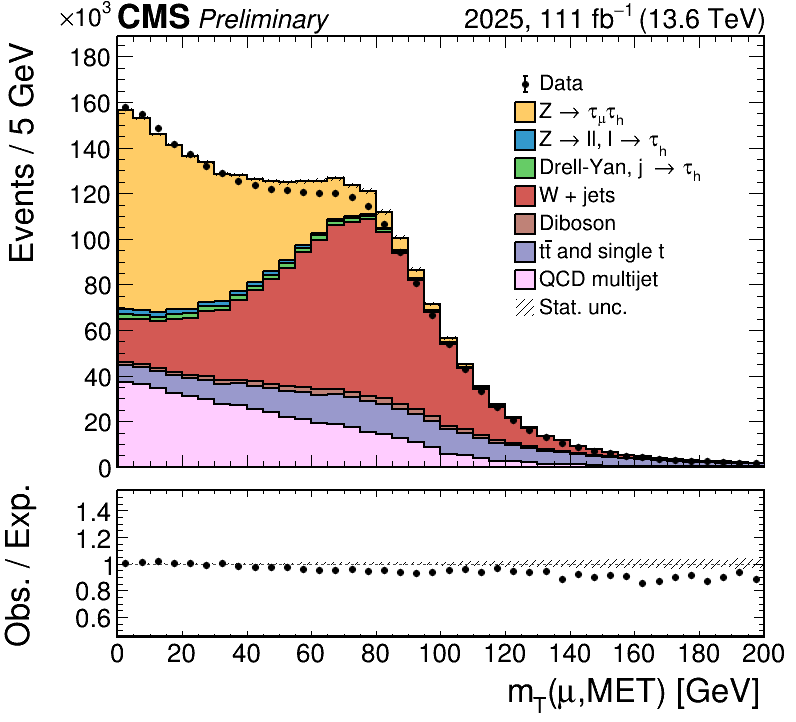
\includegraphics[width=1\linewidth]{figures//chapter_III/mT_2025.png}
%     \caption{Enter Caption}
%     \label{fig:mT_cut_baseline}
% \end{figure}
\begin{figure}
    \centering
    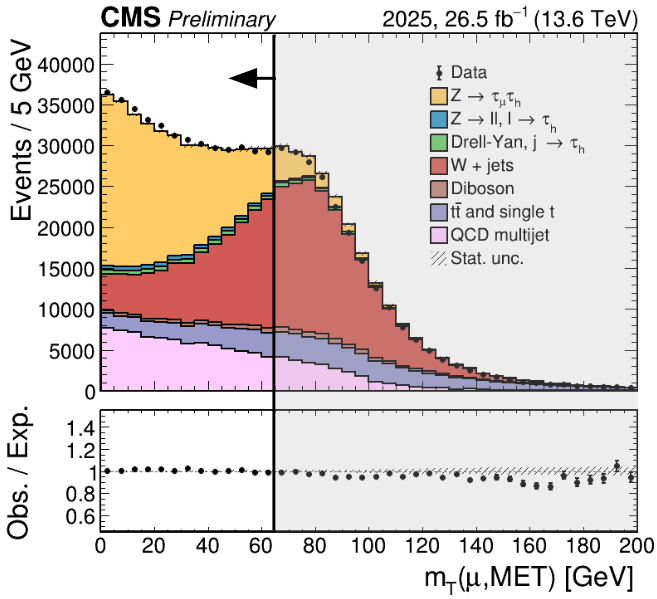
\includegraphics[width=0.5\linewidth]{figures//chapter_III/mT_2025_captura.png}
    \caption{Transverse mass distribution in the $\mu$-MET system, comparing 2025 data with MC simulation. The black line delimits the $Z\rightarrow\tau\tau\rightarrow\mu\tau_h$ enriched signal region below $m_T<65$ GeV, as marked by the arrow. The shaded region indicates the excluded region rich in W+jets contribution, and therefore with a high jet misidentification rate. \textcolor{red}{Hacerla en buena calidad (es screenshot)}}
    \label{fig:mT_cut_baseline}
\end{figure}

Figure \ref{fig:kinematics_mu_tau_2024} shows the simulation-to-data agreement in the signal region, as previously defined, for the kinematic behavior of the reconstructed objects, namely the $\mu$ and the $\tau_h$. To illustrate the validity of the modeling of the reconstructed objects, the distributions in $p_T$, $\eta$ and $\phi$ for both $\mu$ and $\tau_h$ are displayed for a representative year, 2025 in this case. The figure indicate that there are no substantial discrepancies in the shape of the distributions, and the data-to-MC agreement is generally as expected. Minor normalization discrepancies resulting from the absence of dedicated corrections are also anticipated.


\begin{figure}[htbp]
    \centering

    %------------------ ROW 1: MUON ------------------%
    \begin{subfigure}[t]{0.32\linewidth}
        \centering
        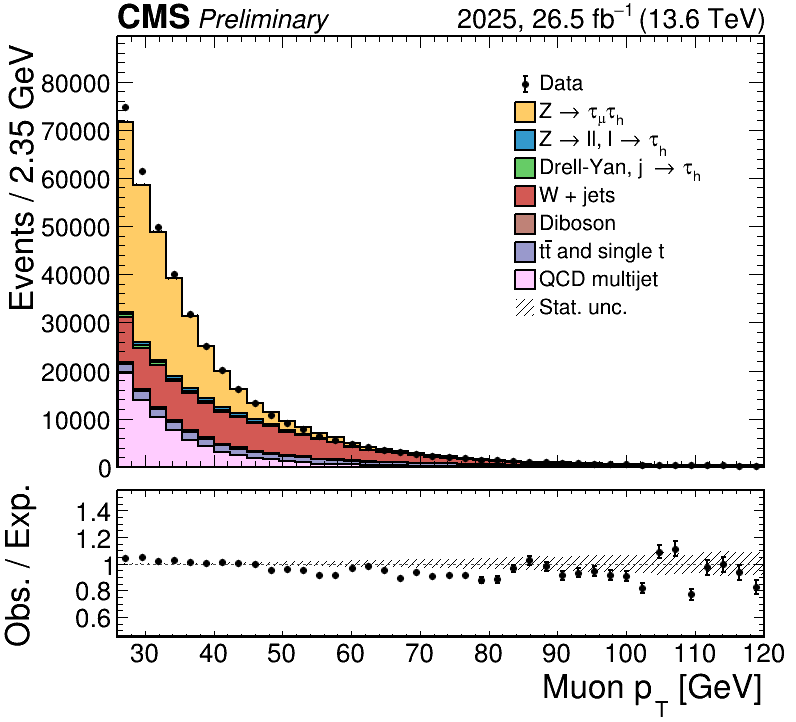
\includegraphics[width=\linewidth]{figures/chapter_III/muon_pt_2025.png}
        \caption{$p_T(\mu)$}
        \label{fig:muon_pt_2024}
    \end{subfigure}
    \hfill
    \begin{subfigure}[t]{0.32\linewidth}
        \centering
        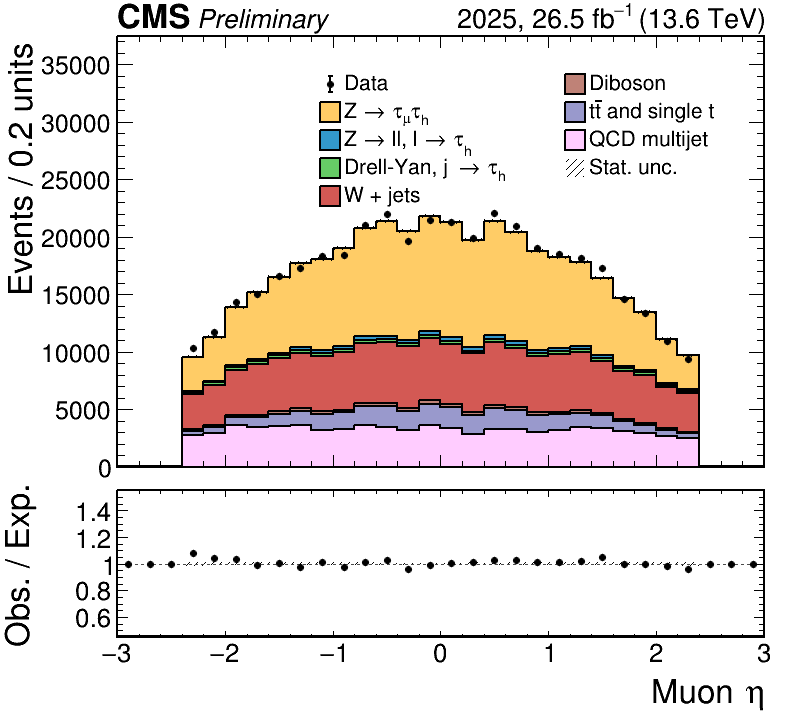
\includegraphics[width=\linewidth]{figures/chapter_III/muon_eta_2025.png}
        \caption{$\eta(\mu)$}
        \label{fig:muon_eta_2024}
    \end{subfigure}
    \hfill
    \begin{subfigure}[t]{0.32\linewidth}
        \centering
        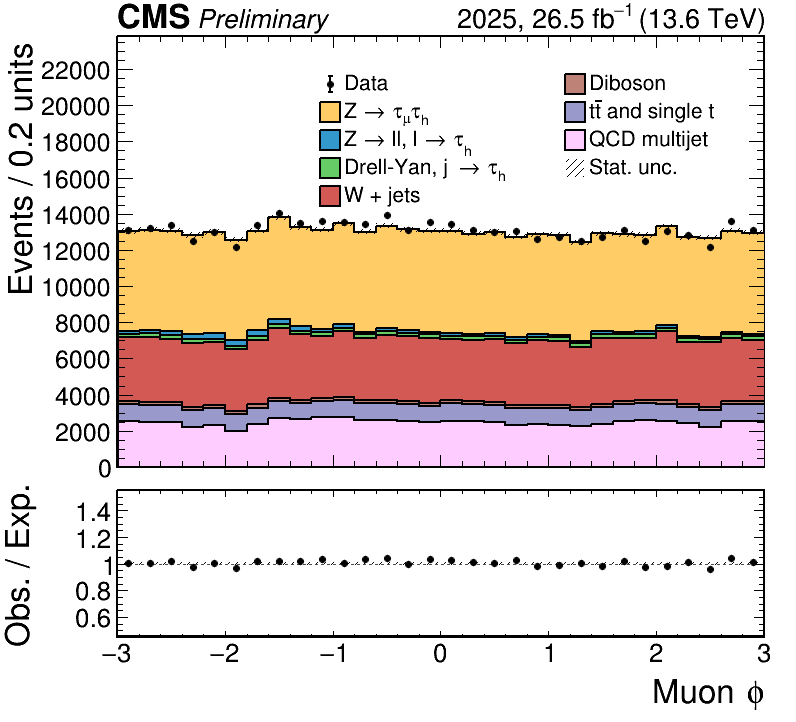
\includegraphics[width=\linewidth]{figures/chapter_III/muon_phi_2025.png}
        \caption{$\phi(\mu)$}
        \label{fig:muon_phi_2024}
    \end{subfigure}

    \vspace{0.5cm}

    %------------------ ROW 2: TAU ------------------%
    \begin{subfigure}[t]{0.32\linewidth}
        \centering
        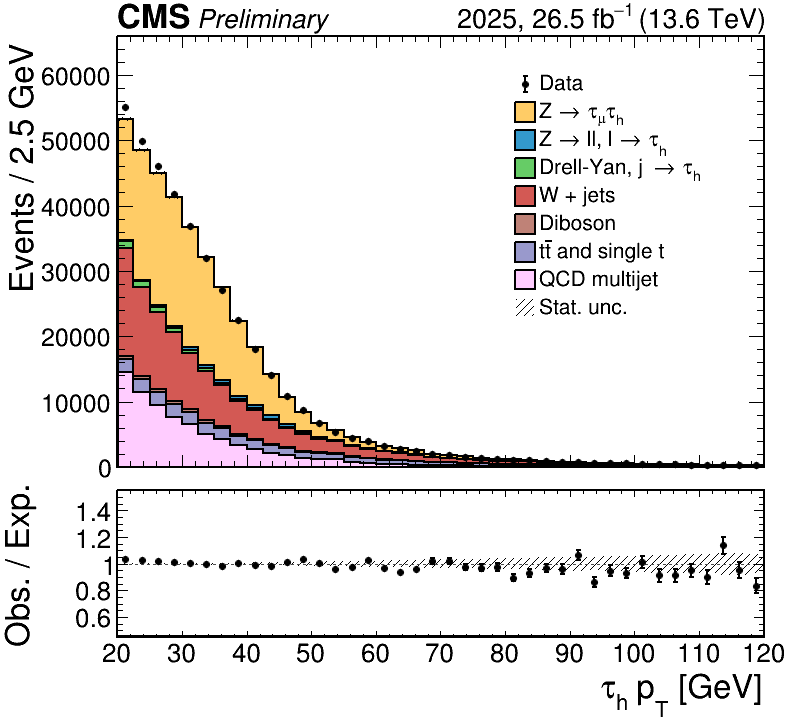
\includegraphics[width=\linewidth]{figures/chapter_III/tau_pt_2025.png}
        \caption{$p_T(\tau_h)$}
        \label{fig:tau_pt_2024}
    \end{subfigure}
    \hfill
    \begin{subfigure}[t]{0.32\linewidth}
        \centering
        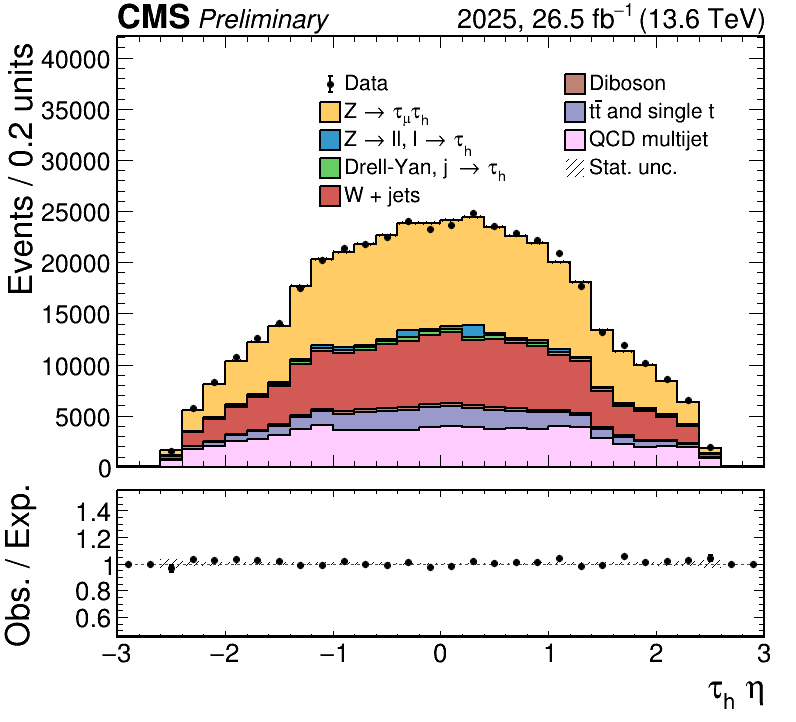
\includegraphics[width=\linewidth]{figures/chapter_III/tau_eta_2025.png}
        \caption{$\eta(\tau_h)$}
        \label{fig:tau_eta_2024}
    \end{subfigure}
    \hfill
    \begin{subfigure}[t]{0.32\linewidth}
        \centering
        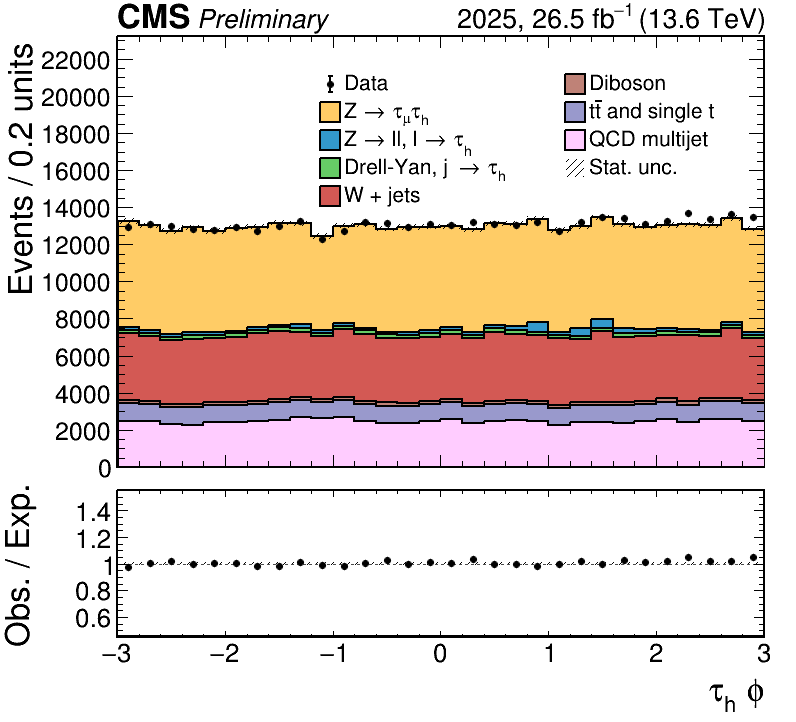
\includegraphics[width=\linewidth]{figures/chapter_III/tau_phi_2025.png}
        \caption{$\phi(\tau_h)$}
        \label{fig:tau_phi_2024}
    \end{subfigure}

    \caption{Comparison between data and simulation for the kinematic distributions of the muon (top row) and the $\tau_h$ candidate (bottom row) in the signal region using 2025 data}
    \label{fig:kinematics_mu_tau_2024}
\end{figure}

The reliability of the $\tau_h$ modeling across the various years of Run-3 is illustrated in Figure \ref{fig:mvis_all_years}. The reference variable used for comparison is the invariant mass of the visible objects in the $\mu\tau_h$ system, $m_{vis}$, since it is a robust observable that is sensitive to possible discrepancies in the $\tau_h$ reconstruction owing to the fact that the behavior of the $\mu$ is widely understood in CMS. The $m_{vis}$ distribution is shown separately for each of the data-taking periods, covering 2022, 2023, 2024, 2025, and 2026. All distributions demonstrate strong data/MC alignment, where the consistency of the shape over the years confirms the good performance in the reconstruction and identification of the $\tau_h$ during Run-3. However, for a more detailed overview, the subsequent Section \ref{subsec:TES_checks} thoroughly examines the stability in the performance of the data collected across the years in terms of relative efficiencies and misidentification rates.
%
%No $\tau_h$-related corrections are applied in these distributions: neither the identification efficiency scale factors nor the energy scale corrections discussed in Section \ref{...}. The residual normalization differences observed in the ratio panels are therefore a direct measure of the size of those corrections, rather than an indication of mismodelling of the $\tau_h$ reconstruction itself.
%
\begin{figure}[htbp]
    \centering

    %------------------ ROW 1 ------------------%
    \begin{subfigure}[t]{0.32\linewidth}
        \centering
        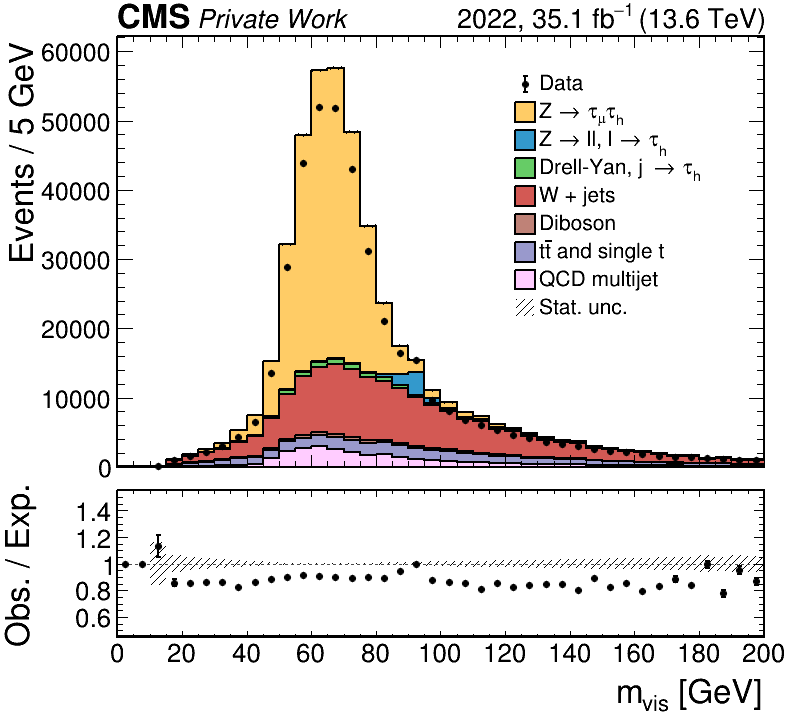
\includegraphics[width=\linewidth]{figures/chapter_III/mvis_2022.png}
        \caption{2022}
        \label{fig:mvis_2022}
    \end{subfigure}
    \hfill
    \begin{subfigure}[t]{0.32\linewidth}
        \centering
        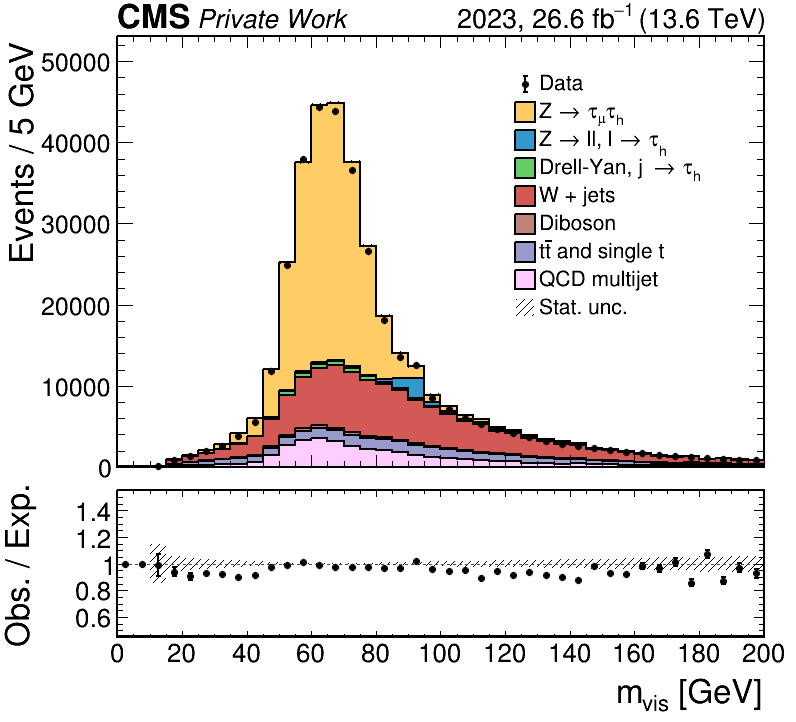
\includegraphics[width=\linewidth]{figures/chapter_III/mvis_2023.png}
        \caption{2023}
        \label{fig:mvis_2023}
    \end{subfigure}
    \hfill
    \begin{subfigure}[t]{0.32\linewidth}
        \centering
        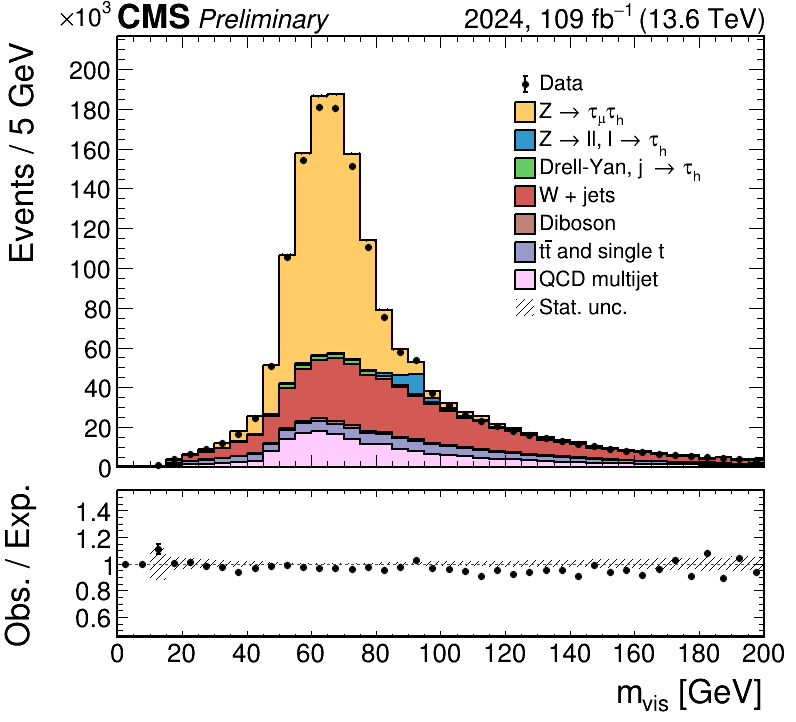
\includegraphics[width=\linewidth]{figures/chapter_III/mvis_DeepTau_2024.png}
        \caption{2024}
        \label{fig:mvis_2024}
    \end{subfigure}

    \vspace{0.6cm}

    %------------------ ROW 2 ------------------%
    \begin{subfigure}[t]{0.32\linewidth}
        \centering
        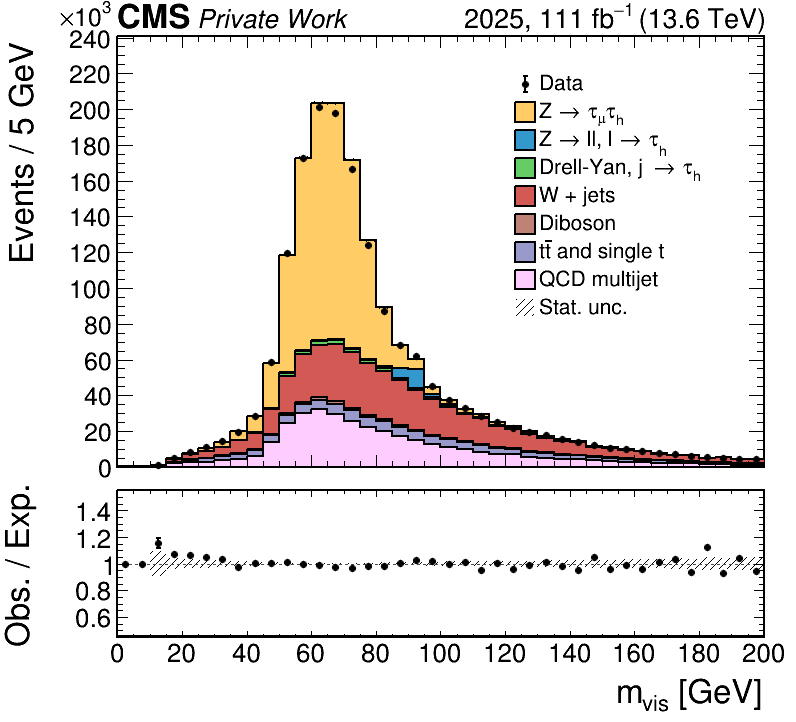
\includegraphics[width=\linewidth]{figures/chapter_III/mvis_DeepTau_2025.png}
        \caption{2025}
        \label{fig:mvis_2025}
    \end{subfigure}
    \hspace{0.03\linewidth} 
    \begin{subfigure}[t]{0.32\linewidth}
        \centering
        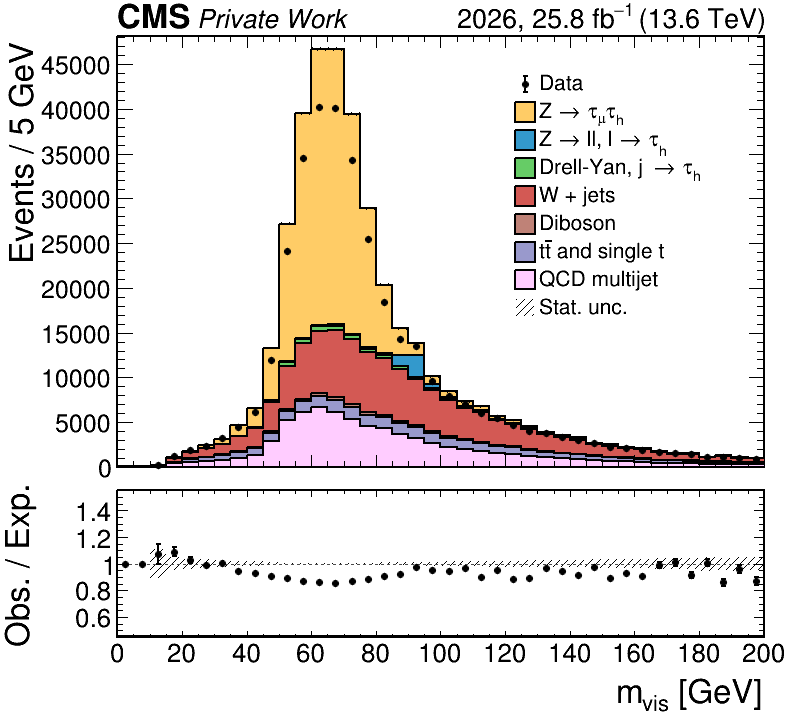
\includegraphics[width=\linewidth]{figures/chapter_III/mvis_2026.png}
        \caption{2026}
        \label{fig:mvis_2026}
    \end{subfigure}

    \caption{Comparison between data and simulation for the visible mass distribution $m_{vis}$ in the signal region for the years 2022 (a), 2023 (b), 2024 (c), 2025 (d) and 2026 (e).}
    \label{fig:mvis_all_years}
\end{figure}


The performance of the aforementioned $\tau_h$ identification algorithms (\textsc{DeepTau v2.5}, \textsc{PNet} and \textsc{UParT}) is compared in Figure \ref{fig:algorithms}, with data from 2024 serving as a reference. The figure illustrates the performance of each classifier through various sets of distribution:

\paragraph{Score distributions:}
The top row of Figure \ref{fig:algorithms} displays the score distributions of the discriminator \textsc{VSjet} returned by each identification algorithm, where the requirement that the $\tau_h$ candidates satisfy the medium \textsc{VSjet} WP has been removed. The range selected for each discriminator score distribution is chosen to ensure the retention of 90\% of the genuine hadronic $\tau$ candidates. The shape of the score distribution for each classifier shows discrepancies linked to the nature of each different architecture. The figure illustrates that the three $\tau_h$ identification algorithms demonstrate strong performance in terms of data-MC agreement, with \textsc{DeepTau} notably outperforming the others due to its domain adaptation feature.
% Since domain adaptation is currently implemented only in \textsc{DeepTau}, the larger data-to-simulation discrepancies observed for \textsc{PNet} and \textsc{UParT} would translate into larger correction factors and associated systematic uncertainties for any analysis adopting them.

\paragraph{Visible mass:}
The middle row serves as an example of the behavior of the visible mass $m_{vis}$ of the system reconstructed using different $\tau_h$ identification algorithms, demonstrating satisfactory simulation-to-data consistency in all cases. As outlined in Section \ref{subsec:tau_IDcomparison}, Figure \ref{fig:algorithms} illustrates how the three identification methods have distinct rejection levels for quark and gluon jets, electrons, and muons, resulting in different yields for each contributing process. Figure \ref{fig:venn_combined} showed the overlap between the algorithms in this regard. Therefore, the combination of two or more of these identification strategies can serve to optimize the selection of genuine $\tau_h$ candidates and the rejection of misidentified objects. This is demonstrated in Figure \ref{fig:mvis_PNetDeepTau_comb}, which shows the visible mass distribution obtained from the combined selection of \textsc{DeepTau v2.5} and \textsc{PNet} algorithms, providing the strongest rejection of misidentified $\tau_h$ candidates.

\paragraph{Decay mode assignment:}
Finally, the set of plots in the last row is intended to illustrate the differences in the assignment of decay modes performed by each algorithm. In these distributions, the $Z\to\mu\tau_h$ signal simulation is separated into its various decay modes to facilitate the visualization of the correct assignment of each decay mode per algorithm under study.

\begin{figure}[htbp]
    \centering

    %------------------ ROW 1: SCORES ------------------%
    \begin{subfigure}[t]{0.32\linewidth}
        \centering
        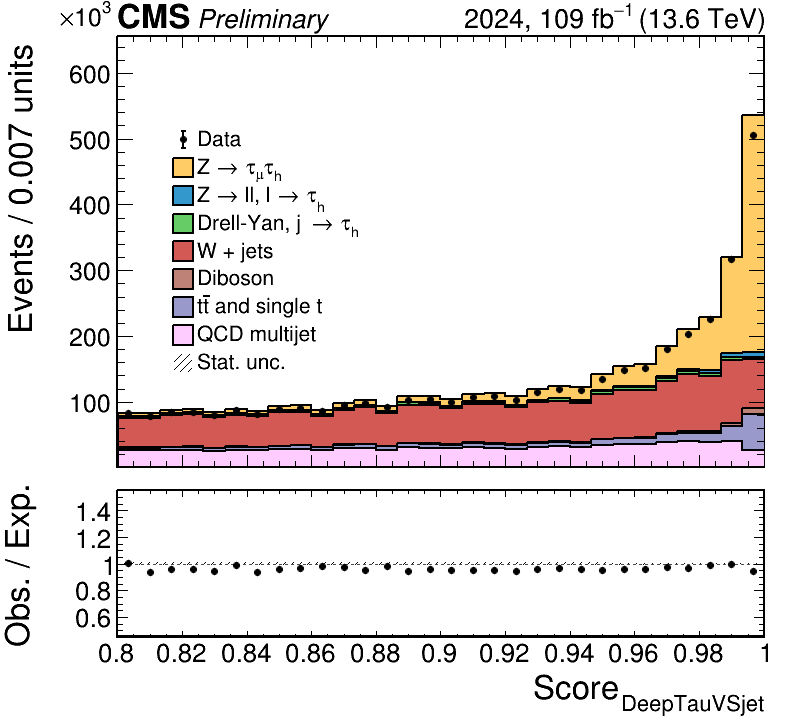
\includegraphics[width=\linewidth]{figures/chapter_III/score_DeepTau_vsJET_2024.png}
        \caption{\textsc{DeepTau v2.5} VSjet score}
        \label{fig:score_deeptau}
    \end{subfigure}
    \hfill
    \begin{subfigure}[t]{0.32\linewidth}
        \centering
        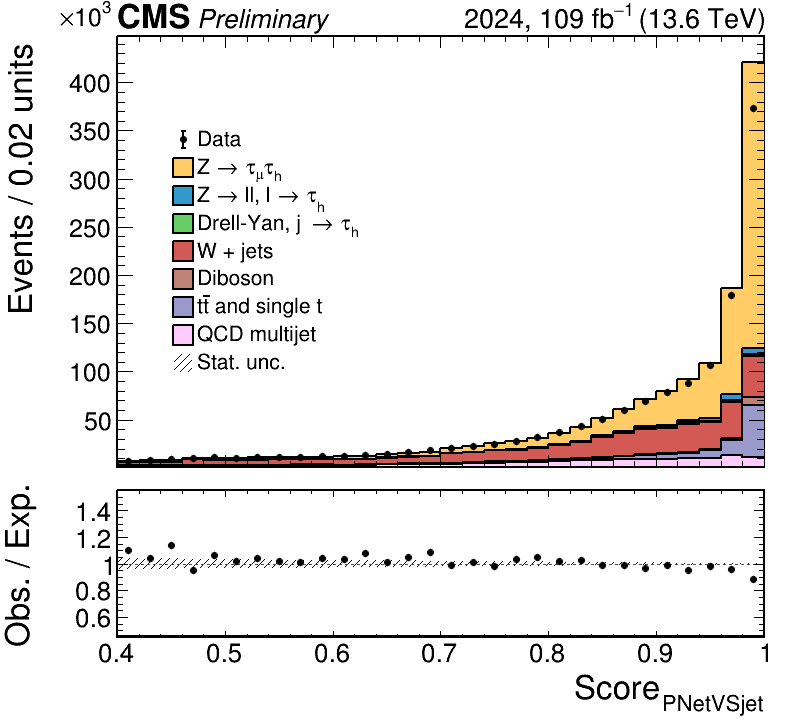
\includegraphics[width=\linewidth]{figures/chapter_III/score_PNet_vsJET_2024.png}
        \caption{\textsc{PNet} VSjet score}
        \label{fig:score_pnet}
    \end{subfigure}
    \hfill
    \begin{subfigure}[t]{0.32\linewidth}
        \centering
        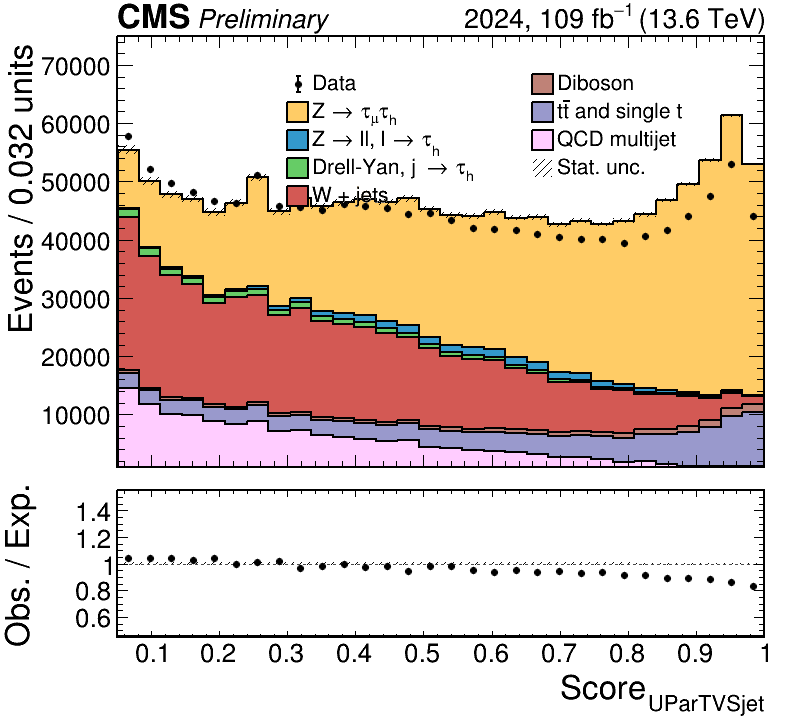
\includegraphics[width=\linewidth]{figures/chapter_III/score_UParT_vsJET_2024.png}
        \caption{\textsc{UParT v2} VSjet score}
        \label{fig:score_upart}
    \end{subfigure}

    \vspace{0.6cm}

    %------------------ ROW 2: MVIS ------------------%
    \begin{subfigure}[t]{0.32\linewidth}
        \centering
        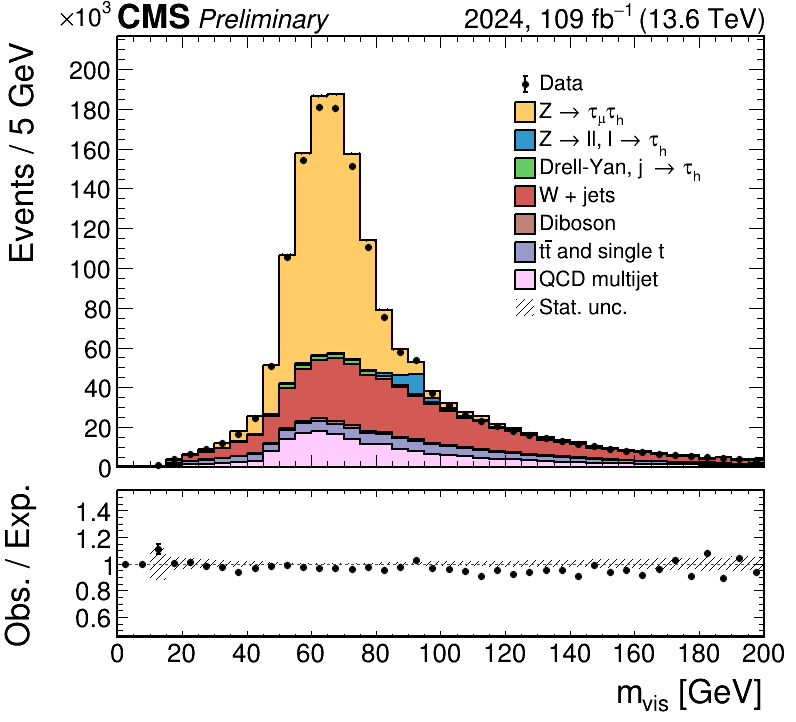
\includegraphics[width=\linewidth]{figures/chapter_III/mvis_DeepTau_2024.png}
        \caption{$m_{\mathrm{vis}}$ (\textsc{DeepTau v2.5})}
        \label{fig:mvis_deeptau}
    \end{subfigure}
    \hfill
    \begin{subfigure}[t]{0.32\linewidth}
        \centering
        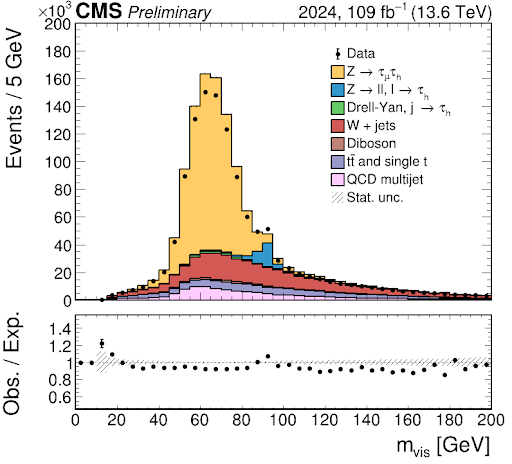
\includegraphics[width=\linewidth]{figures/chapter_III/mvis_PNet_2024.png}
        \caption{$m_{\mathrm{vis}}$ (\textsc{PNet})\textcolor{red}{coger en buena calidad}}
        \label{fig:mvis_pnet}
    \end{subfigure}
    \hfill
    \begin{subfigure}[t]{0.32\linewidth}
        \centering
        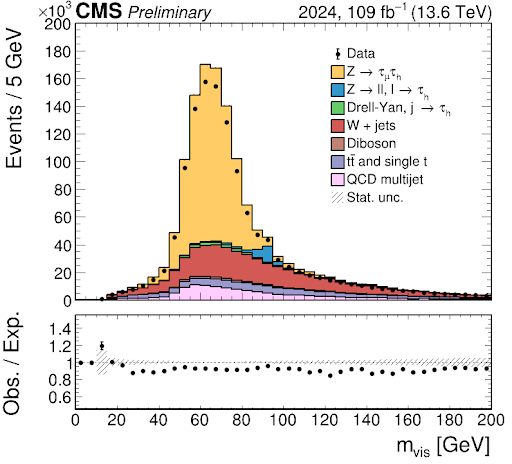
\includegraphics[width=\linewidth]{figures/chapter_III/mvis_UParT_2024.png}
        \caption{$m_{\mathrm{vis}}$ (\textsc{UParT v2})\textcolor{red}{coger en buena calidad}}
        \label{fig:mvis_upart}
    \end{subfigure}

    \vspace{0.6cm}

    %------------------ ROW 3: DECAY MODES ------------------%
    \begin{subfigure}[t]{0.32\linewidth}
        \centering
        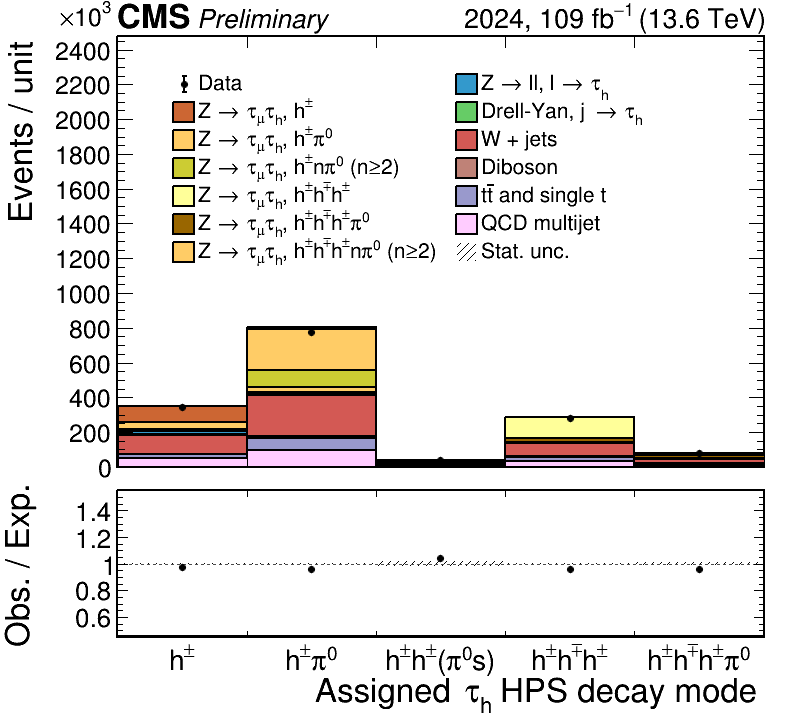
\includegraphics[width=\linewidth]{figures/chapter_III/HPS_DM_2024.png}
        \caption{Decay Mode (HPS)}
        \label{fig:dm_hps}
    \end{subfigure}
    \hfill
    \begin{subfigure}[t]{0.32\linewidth}
        \centering
        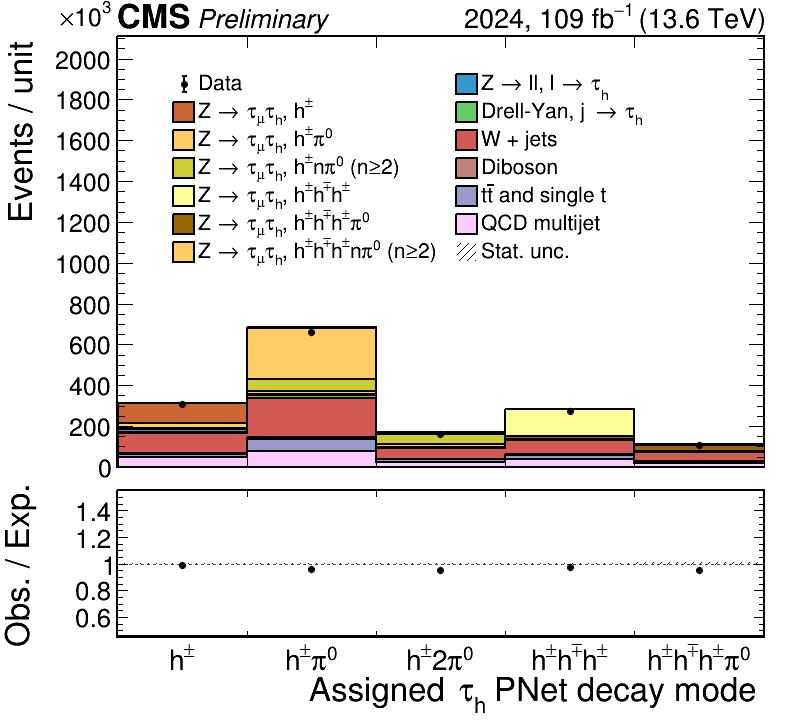
\includegraphics[width=\linewidth]{figures/chapter_III/PNet_DM_2024.png}
        \caption{Decay Mode (\textsc{PNet})}
        \label{fig:dm_pnet}
    \end{subfigure}
    \hfill
    \begin{subfigure}[t]{0.32\linewidth}
        \centering
        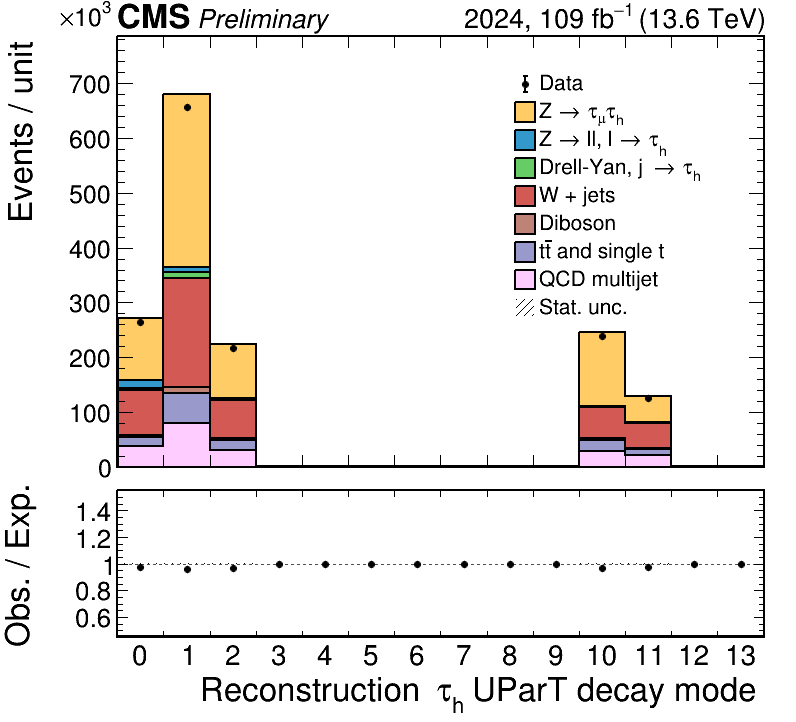
\includegraphics[width=\linewidth]{figures/chapter_III/UParT_DM_2024.png}
        \caption{Decay Mode (\textsc{UParT v2}) \textcolor{red}{REHACER}}
        \label{fig:dm_upart}
    \end{subfigure}

    \caption{
        Summary of the validation of the three $\tau_h$ identification algorithms with 2024 data. 
        \textbf{Top row:} score distributions of the \textsc{VSjet} discriminant for \textsc{DeepTau v2.5}, \textsc{PNet}, and \textsc{UParT v2}. 
        \textbf{Middle row:} visible mass distributions reconstructed with each algorithm. 
        \textbf{Bottom row:} decay mode assigned by each algorithm. 
    }
    \label{fig:algorithms}
\end{figure}

\begin{figure}
    \centering
    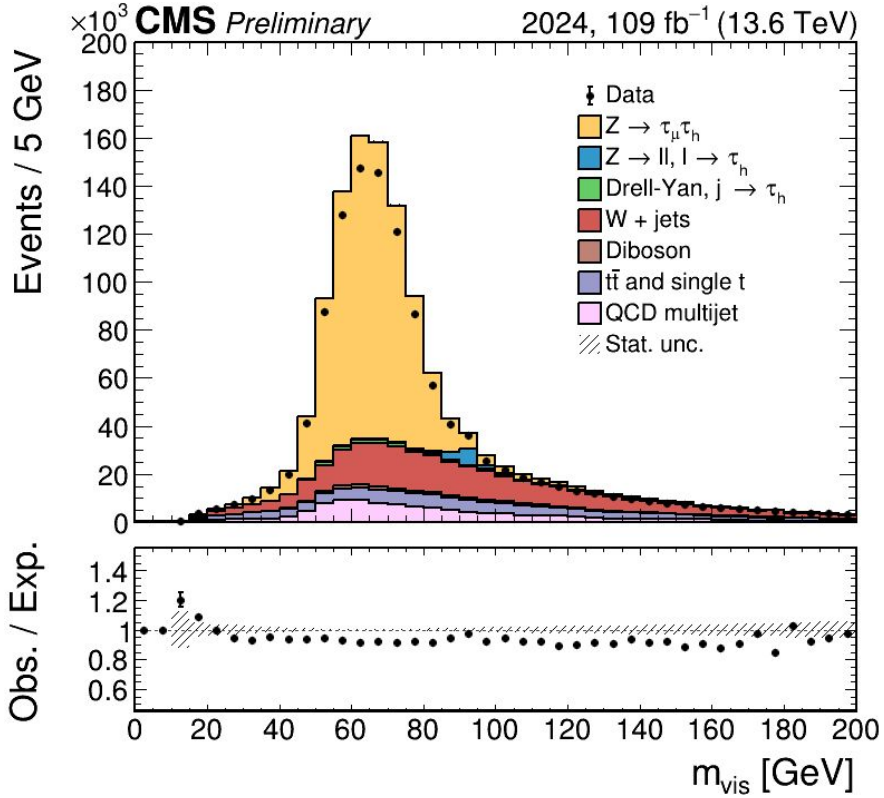
\includegraphics[width=0.6\linewidth]{figures//chapter_III/mvis_DeepTau&PNet.png}
    \caption{Visible mass distribution obtained from the combined selection of \textsc{DeepTau v2.5} and \textsc{PNet}, illustrating the enhanced rejection of misidentified $\tau_h$ candidates achieved when both algorithms are used simultaneously. \textcolor{red}{Es un screenshot, cogerlo en buena calidad}}
    \label{fig:mvis_PNetDeepTau_comb}
\end{figure}

These plots illustrate the difference in classifier response, mass reconstruction, and decay mode assignment across the three identification strategies, and thereby validate the performance of each algorithm in simulation relative to actual data.

\noindent Overall, the evaluation of $\tau_h$ modeling in terms of data-to-MC comparisons has confirmed the robustness of hadronic $\tau$ identification and reconstruction algorithms. To further validate the $\tau$ lepton behavior in CMS, the following section presents the consistency of data collection throughout Run-3, with the aim of addressing possible effects arising from evolving detector conditions.


\subsection{Stability of \texorpdfstring{$\tau_h$}{τh} performance in Run-3 data}
\label{subsec:TES_checks}
%presentación PPD (1): https://indico.cern.ch/event/1569864/contributions/6612866/attachments/3109869/5512492/TauPOG_2024_2025Data_PPD_2407.pdf
%presentación PPD (2): https://docs.google.com/presentation/d/178-DORdl0GOepSjdjDzxOgDB1sgRS6_t_pinHd4K7ro/edit?slide=id.g3c670cd6792_0_1#slide=id.g3c670cd6792_0_1

The previous section presented the Data-to-MC validation, which was designed to verify the correct modeling of $\tau_h$ reconstruction and identification in simulation. This section, in contrast, focuses on evaluating the actual response of the detector throughout the various periods of Run-3. Across these periods, the detector is subject to variations in its operating conditions due to increases in instantaneous luminosity and the aging of the components, which can influence key aspects of $\tau_h$ performance, such as the energy scale, identification efficiency and misidentification rate. Therefore, studying the stability of the collected data becomes imperative to ensure a reliable description of the data through Monte Carlo simulation. These studies thus serve as an independent verification process that complements simulation-based validation. 

The behavior of the data over the years is now addressed using an approach similar to the one presented in previous section. Events from the $Z\to\tau\tau\to\mu\tau_h$ process are selected using data collected with muon triggers and under a preselection criteria analogous to that in Section \ref{subsec:Data-MC-agreement}, with the exception that the $\tau$ must satisfy Tight \textsc{VSjet} WP criterion in order to maximize the purity in genuine $\tau_h$. This is done to ensure that consistency studies actually confirm that any variations across data-taking periods reflect genuine detector effects rather than changes in the background composition. For the studies outlined here, the \textsc{DeepTau} algorithm will be the sole discriminant employed. Furthermore, the cut on the transverse mass $m_T(\mu,MET) < 65$ GeV, as defined in Figure \ref{fig:mT_cut_baseline}, is maintained to preserve a region rich in genuine $\tau_h$ particles.

Figure \ref{figr:data_across_years} shows a comparison of the visible mass of the system $m_{vis}$ over the different periods of Run-3, from 2022 to 2026. Generally, a stable trend is observed across the different data-taking years, with a slight shift observed starting from 2024 onward \textcolor{red}{????}. While deviations of this nature are consistent with the impact of deteriorating detector conditions, they warrant a more detailed investigation of the stability of the data.

\begin{figure}
    \centering
    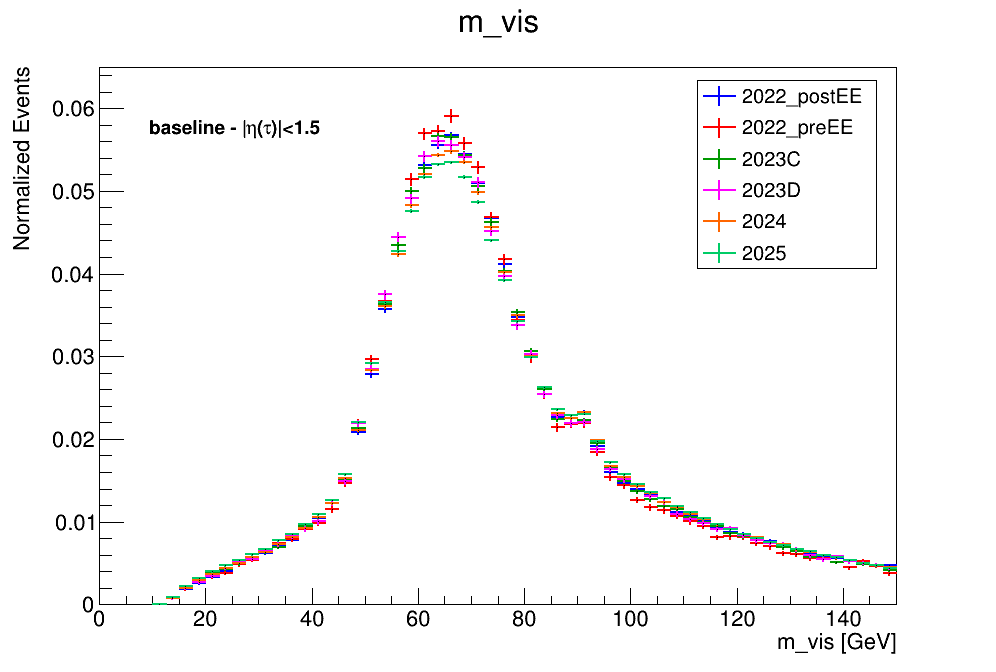
\includegraphics[width=0.5\linewidth]{figures//chapter_III/data_across_years_barrel.png}
    \caption{\textcolor{red}{rehacer el plot para todo eta, añadiendo full 25 + 26 y mejorando el estilo}}
    \label{fig:data_across_years}
\end{figure}

To provide a more detailed characterization of these effects, the visible mass of the $\mu\tau_h$ system in the region enriched with Drell-Yan events is studied. As illustrated in \ref{fig:ratio_plots}, this in-depth study provides valuable insights. The strategy employed consists of plotting the ratio of the $m_{vis}$ distribution across different years for a common reference period that varies for each panel, as explained in more detail in the figure caption. This approach serves to illuminate the distinctions between the various data sets. As a result, different behaviors can be observed:
\begin{itemize}
    \item The $m_{vis}$ region between $40 < m_{vis} < 90$ GeV corresponds to the $Z\to\tau\tau\to\mu\tau_h$ peak and is therefore dominated by genuine hadronic $\tau$ events. This region exhibits consistent behavior over the years, following a flat ratio in all cases, with a minor decline in efficiency towards the end of Run-3, indicating stability in the response of the detector to genuine $\tau_h$.
    \item Outside the $Z\to\tau\tau\to\mu\tau_h$ peak, in the tails of the $m_{vis}$ spectrum, the distribution is dominated by fake $\tau$ particles, primary from jets misidentified as $\tau_h$ in the W+jets background contribution. In these regions, a slight increase in events is observed for 2024, which becomes particularly noticeable in 2025 and 2026, highlighting the greater sensitivty to fakes.
\end{itemize}



%\begin{figure}
%    \centering
%    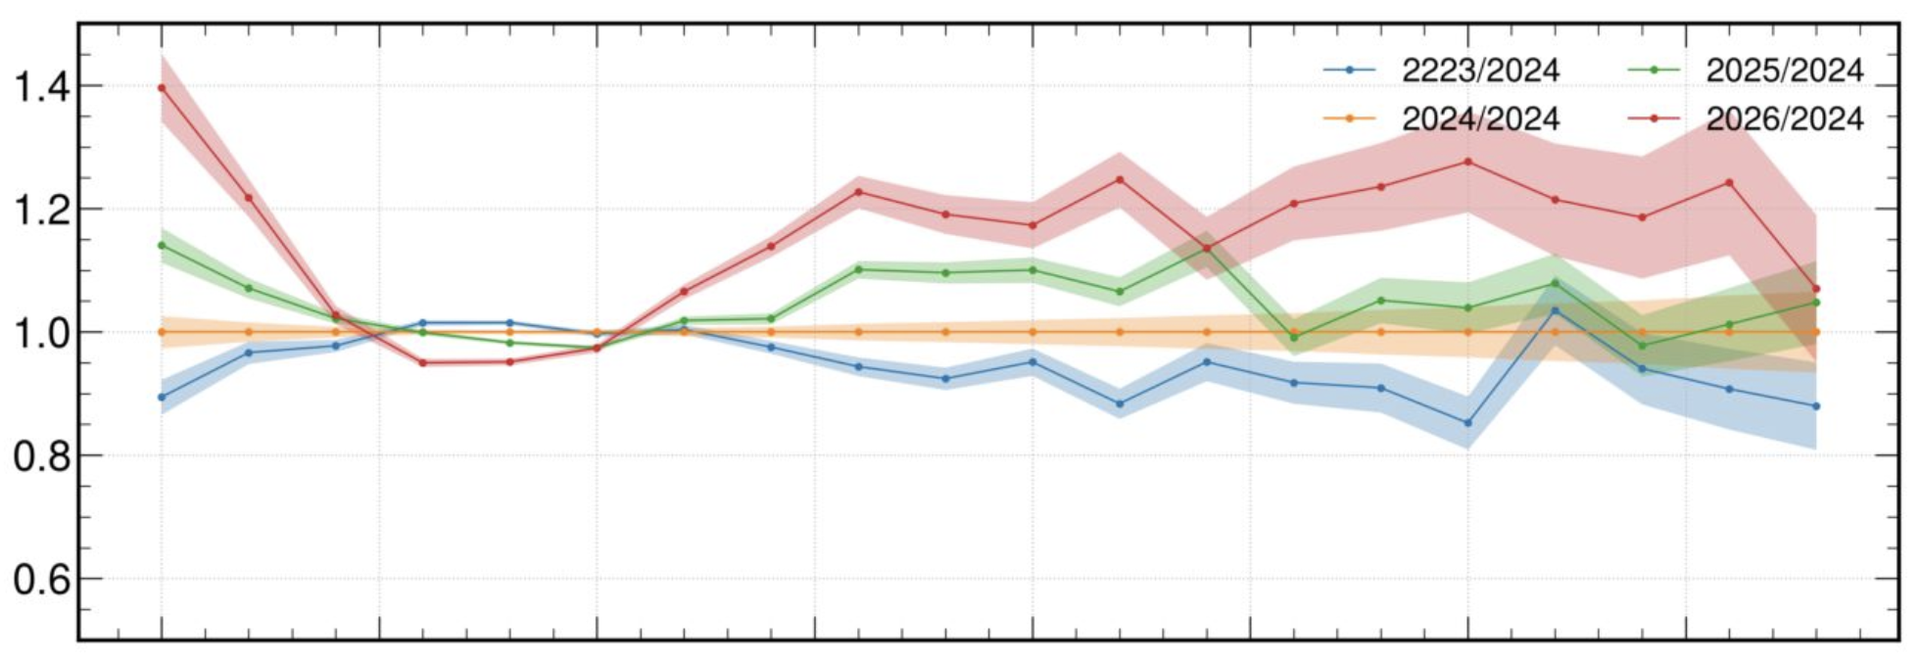
\includegraphics[width=0.5\linewidth]{figures//chapter_III/mvis_ratio_fulldata.png}
%    \caption{\textcolor{red}{estaría bien los plots anteriores pero con todos los años}}
%    \label{fig:placeholder}
%\end{figure}

\begin{figure}
    \centering
    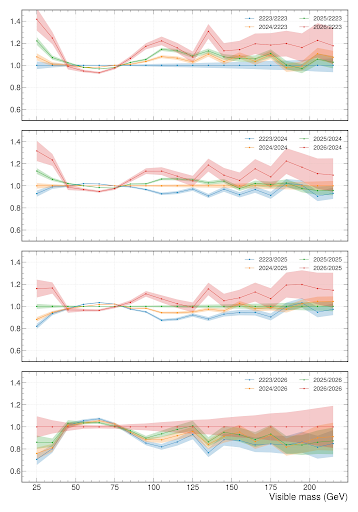
\includegraphics[width=0.5\linewidth]{figures//chapter_III/ratio_DY_2026.png}
    \caption{Ratio of the visible mass $m_{vis}$ distribution in a DY-enriched region across different Run-3 years, shown with respect to a common reference year: the years 2022 and 2023 have been merged as indicated in the figure as 2223 in blue; 2024 in orange; 2025 in blue and 2026 in red. Each panel corresponds to a different reference year, illustrating the evolution of the $m_{vis}$ shape in data between 2022 and 2026. All distributions are normalized to unit area to highlight shape differences only}
    \label{fig:placeholder_2}
\end{figure}

In this way, stability across periods has been verified to account for possible changes in the relative $\tau$ efficiencies, fake rates, and energy scale over the four considered eras. It has been observed that the regions most affected by the different data-acquisition conditions correspond to those dominated by fake $\tau_h$, suchs as events outside the $Z$ mass peak in the DY-enriched region. This indicates that the observed trends stem from variations in the composition and reconstruction of jets misidentified as $\tau_h$ particles, due to detector degradation. Conversely, the response of the detector to authentic hadronic $\tau$ particles remains consistent, validating the stability of the $\tau_h$ energy scale and the efficacy of the reconstruction process throughout the Run-3.

Overall, these stability tests confirm that the performance of the $\tau_h$ in data collected by the detector remains under control across Run-3, with minor variations consistent with the evolution of the detector. This provides an important cross-check of the robustness of the Run-3 $\tau_h$ program.


\vspace{1cm}
\noindent This chapter has demonstrated how the HPS reconstruction and the various identification algorithms — \textsc{DeepTau v2.5}, \textsc{PNet} and \textsc{UParT} — enable the successful identification of the hadronic $\tau$ lepton in experimental collision processes. The focus has been on the various strategies available in CMS, and how the evolution of advanced machine learning techniques, as well as the combination of several of them, enables optimal results to be achieved in discriminating hadronic $\tau$ leptons from various sources of misidentification, while maintaining efficiency for genuine $\tau$ leptons. In addition, the thorough validation process using Run-3 data against Monte Carlo simulations demonstrates the resilience of these algorithms performance under actual detector operating conditions, ensuring reliable and consistent modeling across multiple years. The robustness and confidence provided by the $\tau_h$ program are of great importance for complex physical analyses in final states involving $\tau$ leptons. These elements constitute a fundamental pillar for the study of the $HH\to bb\tau\tau$ channel, which will be discussed in the following chapters.




% Detector holes and hot spots: 
%12.11: https://docs.google.com/presentation/d/15kgMVrNrKn0yoJj5-_G3UvikWLJfFWmZJNiFpdS78qM/edit?slide=id.g2efef749de5_0_3#slide=id.g2efef749de5_0_3
%14.11: https://docs.google.com/presentation/d/1QhgSYqi7aXfBuPNexaYMP5Ko8vo1gtmiUA7vDJvCMOY/edit?slide=id.g3146a045dda_0_0#slide=id.g3146a045dda_0_0